\chapter{Differentation}

\setcounter{section}{8}
\setcounter{subsection}{0}
\setcounter{subsubsection}{1}
\setcounter{secnumdepth}{4}
\subsection{Geometrische Interpretation der Ableitung Teil I u. II}
\href{https://youtu.be/iWT2SWmVfuw}{Video 01}\\
Sei $ f:\mathbb{R}\supset \mathbb{D}_f\longmapsto \mathbb{W}_f\subset\mathbb{R} $ und $ x_0\in \mathbb{D}_f $\\
\begin{center}
	
		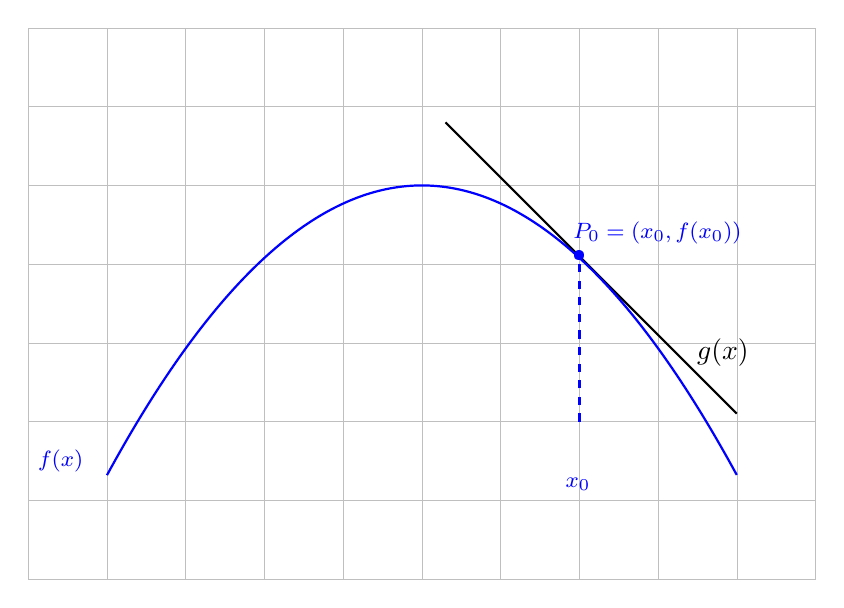
\begin{tikzpicture}
	
	% Gitternetzlinien
	\draw[xstep=1cm, ystep=1cm, very thin, color=lightgray] (-5,5) grid (5,-2);
	% x-Achs
	
	\draw[thick,color=black] plot[samples=200, domain=0.3:4] 
	(\x,{4.1-\x}) node[yshift=2.2em,xshift=-0.5em] {$g(x)$};
	\draw[color=blue] (2,2.1) node {\textbullet};
	
	\draw[thick,color=blue] plot[samples=200, domain=-4:4] 
	(\x,{-0.23*\x*\x+3});
	
	\draw[thick,color=blue,dashed] (2,0) -- (2,2);
	
	\draw[color=blue] (1.8,2.4) node[right] {\footnotesize $P_0=(x_0,f(x_0))$};
	\draw[color=blue] (1.7,-0.8) node[right] {\footnotesize $x_0$};
	\draw[color=blue] (-5,-.5) node[right] {\footnotesize $f(x)$};
	\end{tikzpicture}\\

\end{center}
Die Tangente von $ g $ an $ f $ im Punkt $ P_0 $ soll mit der Geradengleichung dargestellt werden.\\
\begin{align*}
g(x)=mx+n\\
\end{align*}
Die Ableitung von $ f $ in $ x_0 $ ist $ f' (x_0)=m $. Daraus folgt, dass die Steigung der Geraden  bestimmt werden soll.\vspace*{2mm}\\
\newpage
\noindent
Nun wählt man einen zweiten, beliebigen Punkt $P_1\neq P_0 $ auf $ f $ und bildet nun damit eine Sekante.\\
\begin{center}
	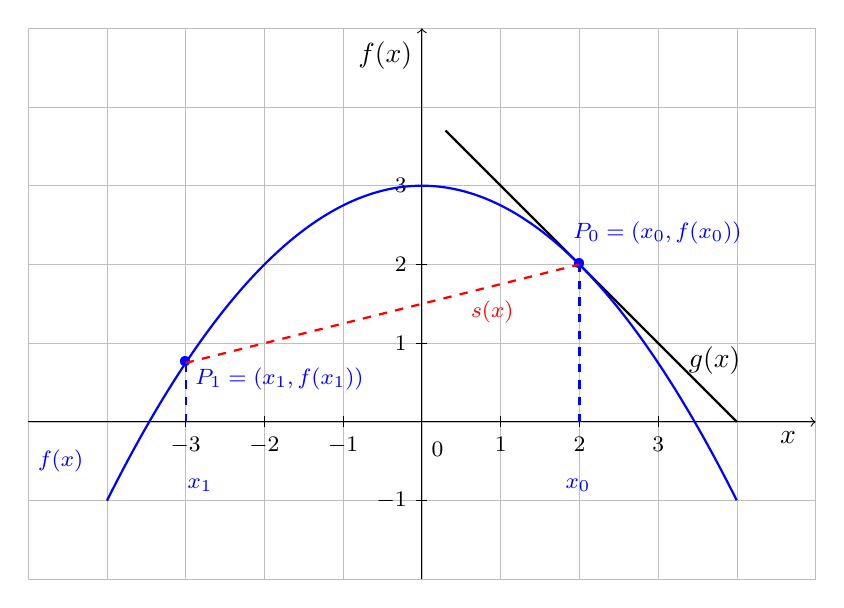
\begin{tikzpicture}
	
	% Gitternetzlinien
	\draw[xstep=1cm, ystep=1cm, very thin, color=lightgray] (-5,5) grid (5,-2);
	% x-Achse
	\draw[->] (-5,0) -- (5,0) node[below,xshift=-1em] {$x$}; 
	%Zahlen auf x-Achse
	\foreach \x in {-3,...,-1}
	\draw[shift={(\x,0)},color=black] (0pt,2pt) -- (0pt,-2pt) node[below] {\footnotesize $\x$};
	\foreach \x in {1,...,3}
	\draw[shift={(\x,0)},color=black] (0pt,2pt) -- (0pt,-2pt) node[below] {\footnotesize $\x$};
	% y-Achse 
	\draw[->] (0,-2) -- (0,5) node[left,yshift=-1em] {$f(x)$};%node[above left]
	%Zahlen auf y-Achse
	\foreach \y in {-1,...,-1}
	\draw[shift={(0,\y)},color=black] (2pt,0pt) -- (-2pt,0pt) node[left] {\footnotesize $\y$};
	\foreach \y in {1,...,3}
	\draw[shift={(0,\y)},color=black] (2pt,0pt) -- (-2pt,0pt) node[left] {\footnotesize $\y$};
	%Ursprung
	\draw[color=black] (0pt,-10pt) node[right] {\footnotesize $0$};
	
	\draw[thick,color=black] plot[samples=200, domain=0.3:4] 
	(\x,{4-\x}) node[yshift=2.2em,xshift=-0.8em] {$g(x)$};
	
	\draw[thick,color=blue] plot[samples=200, domain=-4:4] 
	(\x,{-0.25*\x*\x+3});
	
	\draw[thick,color=blue,dashed] (2,0) -- (2,2);
	\draw[color=blue] (1.8,2.4) node[right] {\footnotesize $P_0=(x_0,f(x_0))$};
	\draw[color=blue] (1.7,-0.8) node[right] {\footnotesize $x_0$};
	
	\draw[color=blue] (2,2) node {\textbullet};
	\draw[thick,color=blue,dashed] (-3,0) -- (-3,0.75);
	\draw[color=blue] (-3.1,-0.8) node[right] {\footnotesize $x_1$};
	\draw[color=blue] (-3,0.75) node {\textbullet};
	
	\draw[color=blue] (-3,0.55) node[right] {\footnotesize $P_1=(x_1,f(x_1))$};
	\draw[thick,color=red,dashed] (-3,0.75) -- (2,2);
	\draw[color=red] (0.5,1.4) node[right] {\footnotesize $s(x)$};
	\draw[color=blue] (-5,-.5) node[right] {\footnotesize $f(x)$};
	\end{tikzpicture}\\	
\end{center}
Bestimmung der Sekante: $ s(x)=mx+n $\\
Es gilt mit $ P_1=(x_1,f(x_1)) $ und $ P_2=(x_0,f(x_0)) $:\\
\begin{align}
f(x_0)=mx_0+n \tag{I}\\
f(x_1)=mx_1+n \tag{II}
\end{align}
Lösung des LGS's.\\
Mit II-I erhält man $ m $.\\
\begin{align*}
&\;\;\;\;\;\;\;\;\;\;\;\;f(x_1)=mx_1+n \\
&\;\;\;\;\;\;\;-(\underline{f(x_0)=mx_0+n })\\
&f(x_1)-f(x_0)=mx_1-mx_0\\
&f(x_1)-f(x_0)=m(x_1-x_0)\\
&\Leftrightarrow\\
&m=\frac{f(x_1)-f(x_0)}{x_1-x_0}\\
\end{align*}
Durch Einsetzen von $ m $ in I erhält man $ n $.\\
\begin{align*}
&f(x_0)=\frac{f(x_1)-f(x_0)}{x_1-x_0}\cdot x_0+n\\
&\Leftrightarrow\\
&n=f(x_0)-\frac{f(x_1)-f(x_0)}{x_1-x_0}\cdot x_0\\
\end{align*}
Durch einsetzen von $ n,m $ in $ s(x)=mx+n $ erhält man $ s(x) $:
\begin{align*}
s(x)&=\frac{f(x_1)-f(x_0)}{x_1-x_0}\cdot x+f(x_0)-\frac{f(x_1)-f(x_0)}{x_1-x_0}\cdot x_0\\
s(x)&=f(x_0)+\frac{f(x_1)-f(x_0)}{x_1-x_0}\cdot(x-x_0)
\end{align*}
Das Ziel ist jetzt, eine geschlossene Formel für die Steigung $ m $ zu finden.\\
Die Idee ist:\\
Den Punkt $ P_1 $ entlang der Kurve von $ f(x) $ zum Punkt $ P_0 $ laufen zu lassen.\\
\begin{center}
	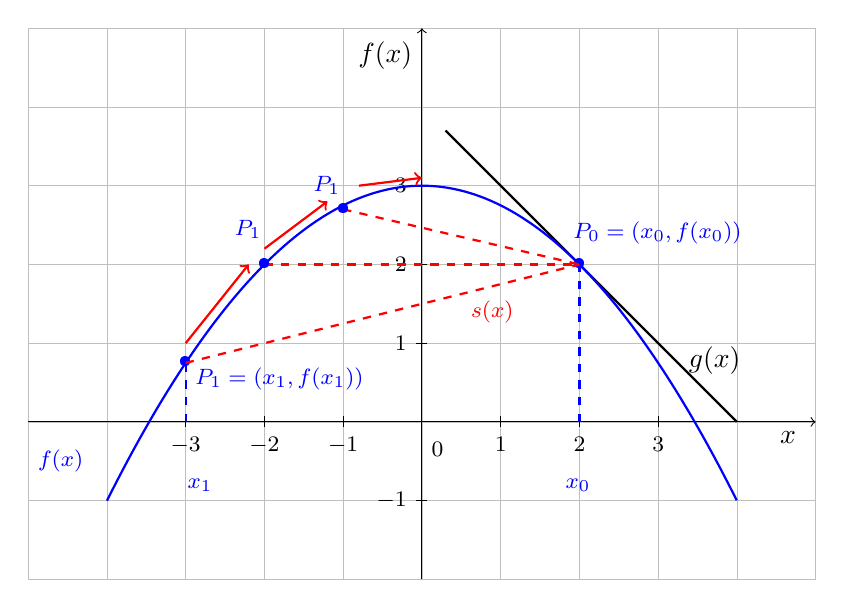
\begin{tikzpicture}
	
	% Gitternetzlinien
	\draw[xstep=1cm, ystep=1cm, very thin, color=lightgray] (-5,5) grid (5,-2);
	% x-Achse
	\draw[->] (-5,0) -- (5,0) node[below,xshift=-1em] {$x$}; 
	%Zahlen auf x-Achse
	\foreach \x in {-3,...,-1}
	\draw[shift={(\x,0)},color=black] (0pt,2pt) -- (0pt,-2pt) node[below] {\footnotesize $\x$};
	\foreach \x in {1,...,3}
	\draw[shift={(\x,0)},color=black] (0pt,2pt) -- (0pt,-2pt) node[below] {\footnotesize $\x$};
	% y-Achse 
	\draw[->] (0,-2) -- (0,5) node[left,yshift=-1em] {$f(x)$};%node[above left]
	%Zahlen auf y-Achse
	\foreach \y in {-1,...,-1}
	\draw[shift={(0,\y)},color=black] (2pt,0pt) -- (-2pt,0pt) node[left] {\footnotesize $\y$};
	\foreach \y in {1,...,3}
	\draw[shift={(0,\y)},color=black] (2pt,0pt) -- (-2pt,0pt) node[left] {\footnotesize $\y$};
	%Ursprung
	\draw[color=black] (0pt,-10pt) node[right] {\footnotesize $0$};
	
	\draw[thick,color=black] plot[samples=200, domain=0.3:4] 
	(\x,{4-\x}) node[yshift=2.2em,xshift=-0.8em] {$g(x)$};
	
	\draw[thick,color=blue] plot[samples=200, domain=-4:4] 
	(\x,{-0.25*\x*\x+3});
	
	\draw[thick,color=blue,dashed] (2,0) -- (2,2);
	\draw[color=blue] (1.8,2.4) node[right] {\footnotesize $P_0=(x_0,f(x_0))$};
	\draw[color=blue] (1.7,-0.8) node[right] {\footnotesize $x_0$};
	
	\draw[color=blue] (2,2) node {\textbullet};
	\draw[thick,color=blue,dashed] (-3,0) -- (-3,0.75);
	\draw[color=blue] (-3.1,-0.8) node[right] {\footnotesize $x_1$};
	\draw[color=blue] (-3,0.75) node {\textbullet};
	
	\draw[color=blue] (-3,0.55) node[right] {\footnotesize $P_1=(x_1,f(x_1))$};
	\draw[thick,color=red,dashed] (-3,0.75) -- (2,2);
	\draw[color=red] (0.5,1.4) node[right] {\footnotesize $s(x)$};
	\draw[thick,color=red,dashed] (-2,2) -- (2,2);
	\draw[color=blue] (-2,2) node {\textbullet};
	\draw[color=blue] (-2.5,2.45) node[right] {\footnotesize $P_1$};
	\draw[thick,color=red,->] (-3,1) -- (-2.2,2);	
	\draw[thick,color=red,dashed] (-1,2.7) -- (2,2);
	\draw[color=blue] (-1,2.7) node {\textbullet};
	\draw[color=blue] (-1.5,3) node[right] {\footnotesize $P_1$};
	\draw[thick,color=red,->] (-0.8,3) -- (0,3.1);	
	\draw[thick,color=red,->] (-2,2.2) -- (-1.2,2.8);
	\draw[color=blue] (-5,-.5) node[right] {\footnotesize $f(x)$};
	\end{tikzpicture}\\	
\end{center}
Dann gilt, wenn $ f(x) $ bis zu $ f(x_0) $ geht:\\
\begin{align*}
\lim\limits_ {x_1\to x_0}\frac{f(x_1)-f(x_0)}{x_1-x_0}=m=f'(x_0)\\
\end{align*}
\href{https://youtu.be/TlYjfC4L394}{Video 02}\\
Natürlich kann man ein beliebiges $ x_1 $ wählen, also gilt dann:\\
\begin{align*}
\lim\limits_ {x\to x_0}\frac{f(x)-f(x_0)}{x-x_0}=m=f'(x_0)\\
\end{align*}
Überlegungen:\\
\begin{center}
	
	
	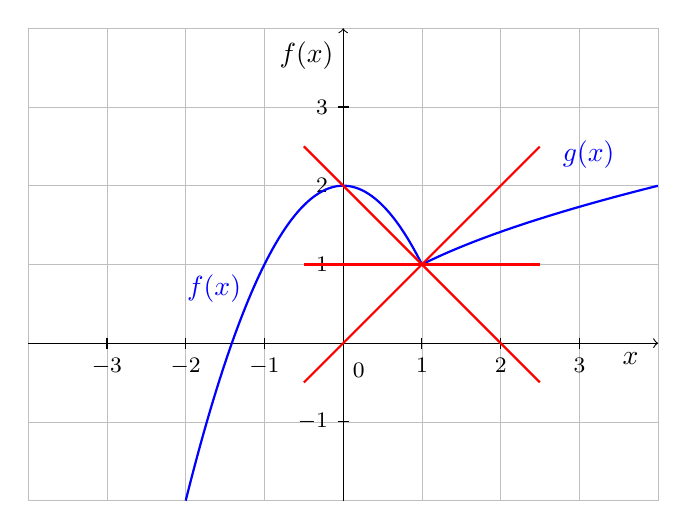
\begin{tikzpicture}
	
	% Gitternetzlinien
	\draw[xstep=1cm, ystep=1cm, very thin, color=lightgray] (-4,4) grid (4,-2);
	% x-Achse
	\draw[->] (-4,0) -- (4,0) node[below,xshift=-1em] {$x$}; 
	%Zahlen auf x-Achse
	\foreach \x in {-3,...,-1}
	\draw[shift={(\x,0)},color=black] (0pt,2pt) -- (0pt,-2pt) node[below] {\footnotesize $\x$};
	\foreach \x in {1,...,3}
	\draw[shift={(\x,0)},color=black] (0pt,2pt) -- (0pt,-2pt) node[below] {\footnotesize $\x$};
	% y-Achse 
	\draw[->] (0,-2) -- (0,4) node[left,yshift=-1em] {$f(x)$};%node[above left]
	%Zahlen auf y-Achse
	\foreach \y in {-1,...,-1}
	\draw[shift={(0,\y)},color=black] (2pt,0pt) -- (-2pt,0pt) node[left] {\footnotesize $\y$};
	\foreach \y in {1,...,3}
	\draw[shift={(0,\y)},color=black] (2pt,0pt) -- (-2pt,0pt) node[left] {\footnotesize $\y$};
	%Ursprung
	\draw[color=black] (0pt,-10pt) node[right] {\footnotesize $0$};
	
	\draw[thick,color=blue] plot[samples=200, domain=1:4] 
	(\x,{sqrt(\x)}) node[below, xshift=-2.5em,yshift=2em] {$g(x)$};
	
	\draw[thick,color=blue] plot[samples=200, domain=-2:1] 
	(\x,{-\x*\x+2}) node[below, xshift=-75]{$f(x)$};
	\draw[thick,color=red] plot[samples=200, domain=-0.5:2.5] 
	(\x,{\x});
	\draw[thick,color=red] plot[samples=200, domain=-0.5:2.5] 
	(\x,{-\x+2});
	\draw[thick,color=red] plot[samples=200, domain=-0.5:2.5] 
	(\x,{1});
	\end{tikzpicture}\\
\end{center}
An dieser Spitze können beliebig viele Tangenten angelegt werden. Der Grenzwert ist hier nicht eindeutig. Er existiert hier nicht.\vspace*{4mm}\\
Polstelle:\\
\begin{center}
	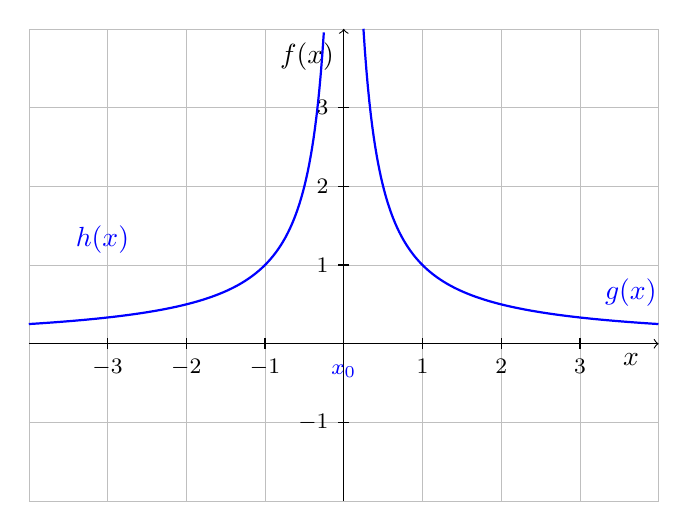
\begin{tikzpicture}
	
	% Gitternetzlinien
	\draw[xstep=1cm, ystep=1cm, very thin, color=lightgray] (-4,4) grid (4,-2);
	% x-Achse
	\draw[->] (-4,0) -- (4,0) node[below,xshift=-1em] {$x$}; 
	%Zahlen auf x-Achse
	\foreach \x in {-3,...,-1}
	\draw[shift={(\x,0)},color=black] (0pt,2pt) -- (0pt,-2pt) node[below] {\footnotesize $\x$};
	\foreach \x in {1,...,3}
	\draw[shift={(\x,0)},color=black] (0pt,2pt) -- (0pt,-2pt) node[below] {\footnotesize $\x$};
	% y-Achse 
	\draw[->] (0,-2) -- (0,4) node[left,yshift=-1em] {$f(x)$};%node[above left]
	%Zahlen auf y-Achse
	\foreach \y in {-1,...,-1}
	\draw[shift={(0,\y)},color=black] (2pt,0pt) -- (-2pt,0pt) node[left] {\footnotesize $\y$};
	\foreach \y in {1,...,3}
	\draw[shift={(0,\y)},color=black] (2pt,0pt) -- (-2pt,0pt) node[left] {\footnotesize $\y$};
	%Ursprung
	\draw[color=blue] (0pt,-10pt) node {\footnotesize $x_0$};
	
	\draw[thick,color=blue] plot[samples=200, domain=-4:-0.25] 
	(\x,{1/abs(\x)}) node[below, yshift=-6.6em,xshift=-8em] {$h(x)$};
	
	\draw[thick,color=blue] plot[samples=200, domain=0.25:4] 
	(\x,{1/\x}) node[below, yshift=2em,xshift=-1em]{$g(x)$};
	
	
	
	\end{tikzpicture}\\
\end{center}
Bei $ x_0 $ kann keine Tangente angelegt werden. Die Funkton ist hier nicht differenzierbar.\\
Der Grenzwert geht gegen $ +\infty $. Geometrisch könnte man sich eine Tangente parallel zur y-Achse vorstellen.\\
\subsection{Differenzierbarkeit}
\href{https://youtu.be/RvEYe71qW_w}{Video 03}\\
Definition:\\
$f:\mathbb{R}\supset I\longmapsto\mathbb{R}$ heißt in $ x_0\in I $ differenzierbar, wenn dieser Differentialquotient existiert.\\
\begin{align*}
\lim\limits_ {x\to x_0}\frac{f(x)-f(x_0)}{x-x_0}=f'(x_0)\in \mathbb{R}\\
\end{align*}
Man nennt $ f'(x_0) $ die Ableitung von $ f $ in $ x_0\in I $.\\
Die Funktion $ f $ ist auf der Menge $I$ diffbar, wenn $ f $ in jedem $ x\in I $ diffbar ist.\vspace*{2mm}\\
Beispiel:\\
Die Funktion $ f:\mathbb{R}\longmapsto [0,\infty[ $ mit $ x\longmapsto x^2 $ ist in $ x_0 $ diffbar.\\
Denn der\\
\begin{align*}
\lim\limits_ {x\to 0}\frac{f(x)-f(x_0)}{x-x_0}=\lim\limits_ {x\to 0}\frac{x^2-0^2}{x-0}=\lim\limits_ {x\to 0}\frac{x^2}{x}=\lim\limits_ {x\to 0}x=0=f'(0)\\
\end{align*}
Allgemein für $ x_0\in \mathbb{R} $ beliebig gilt:\\
\begin{align*}
\lim\limits_ {x\to 0}\frac{f(x)-f(x_0)}{x-x_0}=\lim\limits_ {x\to 0}\frac{x^2-x_0^2}{x-x_0}=\lim\limits_ {x\to 0}\frac{(x-x_0)(x+x_0)}{x-x_0}=\lim\limits_ {x\to x_0}x+x_0=x_0+x_0=2x_0=f'(x_0)\\
\end{align*}
Da die $ 2\in \mathbb{R} $ (von $2x_0=f'(x_0)$ )ist, gilt:\\
$ f $ ist für alle $ x\in \mathbb{R} $ diffbar mit $ f' (x)=(x^2)'=2\cdot x$\\
\newpage
\noindent
\subsubsection{Aufgabe zur Differenzierbarkeit}
\href{https://youtu.be/xyC4rGxDFrM}{Video 04}\\
Zeige, dass $ f:[0,\infty[ \;\;\longmapsto[0,\infty[$ mit $ f(x)=\sqrt{x} $ auf $ ]0,\infty[ $ diffbar ist und berechne $ f'(x) $.\vspace*{2mm}\\
Betrachte den Grenzwert: \\
\begin{align*}
\lim\limits_ {x\to x_0}\frac{f(x)-f(x_0)}{x-x_0}\;\;\text{für }\;\; x_0\in \;]0,\infty[ \\
\end{align*}
\begin{align*}
\lim\limits_ {x\to x_0}\frac{f(x)-f(x_0)}{x-x_0} &=\lim\limits_ {x\to x_0}\frac{\sqrt{x}-\sqrt{x_0}}{x-x_0}\\
&=\lim\limits_ {x\to x_0}\frac{(\sqrt{x}+\sqrt{x_0})(\sqrt{x}-\sqrt{x_0})}{(\sqrt{x}+\sqrt{x_0})(x-x_0)}\\
&=\lim\limits_ {x\to x_0}\frac{x-x_0}{(\sqrt{x}+\sqrt{x_0})(x-x_0)}\\
&=\lim\limits_ {x\to x_0}\frac{1}{\sqrt{x}+\sqrt{x_0}}\\
&=\frac{1}{\sqrt{x_0}+\sqrt{x_0}}\\
&=\underbrace{\frac{1}{2\sqrt{x_0}}}_{\in \mathbb{R}}=f'(x_0)
\end{align*}
D.h. der Grenzwert für $\lim\limits_ {x\to x_0}\frac{f(x)-f(x_0)}{x-x_0}  $ existiert und so gilt:\\
\begin{align*}
f'=(\sqrt{x})'=\frac{1}{2\sqrt{x}}\;\;\text{für }\;\; x\in \;]0,\infty[\\
\end{align*}
Bei Null existiert kein Grenzwert, weil von links kein Grenzwert berechnet werden kann.\\
\begin{align*}
\lim\limits_ {\substack{x \to 0 \\ x<0}}=\frac{1}{2\sqrt{x}}\;\;\text{geht nicht, weil nicht definiert!! }
\end{align*}
Geometrisch gedeutet:\\
\begin{center}
	
	
	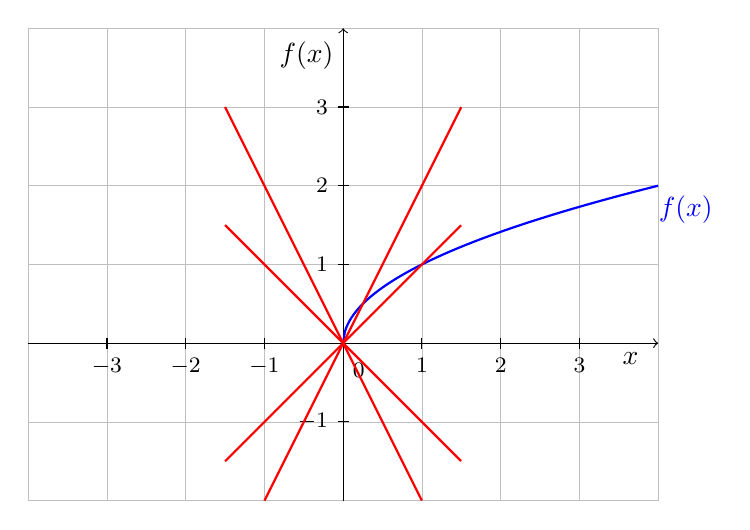
\begin{tikzpicture}
	
	% Gitternetzlinien
	\draw[xstep=1cm, ystep=1cm, very thin, color=lightgray] (-4,4) grid (4,-2);
	% x-Achse
	\draw[->] (-4,0) -- (4,0) node[below,xshift=-1em] {$x$}; 
	%Zahlen auf x-Achse
	\foreach \x in {-3,...,-1}
	\draw[shift={(\x,0)},color=black] (0pt,2pt) -- (0pt,-2pt) node[below] {\footnotesize $\x$};
	\foreach \x in {1,...,3}
	\draw[shift={(\x,0)},color=black] (0pt,2pt) -- (0pt,-2pt) node[below] {\footnotesize $\x$};
	% y-Achse 
	\draw[->] (0,-2) -- (0,4) node[left,yshift=-1em] {$f(x)$};%node[above left]
	%Zahlen auf y-Achse
	\foreach \y in {-1,...,-1}
	\draw[shift={(0,\y)},color=black] (2pt,0pt) -- (-2pt,0pt) node[left] {\footnotesize $\y$};
	\foreach \y in {1,...,3}
	\draw[shift={(0,\y)},color=black] (2pt,0pt) -- (-2pt,0pt) node[left] {\footnotesize $\y$};
	%Ursprung
	\draw[color=black] (0pt,-10pt) node[right] {\footnotesize $0$};
	
	
	
	\draw[thick,color=blue] plot[samples=200, domain=0:4] 
	(\x,{sqrt(\x)}) node[below, xshift=1em]{$f(x)$};
	
	\draw[thick,color=red] plot[samples=200, domain=-1.5:1.5] 
	(\x,{\x});
	\draw[thick,color=red] plot[samples=200, domain=-1.5:1] 
	(\x,{-2*\x});
	\draw[thick,color=red] plot[samples=200, domain=-1.5:1.5] 
	(\x,{-\x});
	\draw[thick,color=red] plot[samples=200, domain=-1:1.5] 
	(\x,{2*\x});
	\end{tikzpicture}\\
\end{center}
Bei Null können beliebig viele Tangenten angelegt werden.\\
\subsection{Stetigkeit und Differenzierbarkeit}
\href{https://youtu.be/Dx6XH3DJ3GA}{Video 05}\\
Satz:\\
\begin{center}
	\boxed{\text{Jede differenzierbare Funktion ist stetig. }}\\
\end{center}
Beispiel:\\
\textbullet\;\;$ f:\mathbb{R}\longmapsto [o,\infty[ $ mit $ f(x)=x^2 $\\
\begin{quote}
	Diese Funktion ist für alle $ x\in \mathbb{R} $ diffbar also auch in allen $ x\in \mathbb{R} $ stetig.\vspace*{2mm}\\
	Bemerkung:\\
	Ist eine Funktion diffbar dann ist sie auch stetig. So kann auch eine Stetigkeit überprüft werden.\vspace*{2mm}\\
	
\end{quote}
\textbullet\;\;$ f:\mathbb{R}\longmapsto[o,\infty[ $ mit $ f(x) = |x|    \left\{ \begin{array}{rcl}
x & \mbox{für} & x\geq0\\
-x & \mbox{für} & x<0 \\

\end{array}\right. $
\begin{quote}
	$\blacktriangleright$ Grenzwert in $ x_0=0 $ bestimmen:\\
	\begin{align*}
	&\lim\limits_ {\substack{x \to 0 \\ x<0}}|x|=\lim\limits_ {x\to 0}=0=\lim\limits_ {x\to 0}=\lim\limits_ {\substack{x \to 0 \\ x>0}}|x|\\
	&\Rightarrow |x| \;\;\text{in }\;\;x_0=0\;\;\text{stetig }\\
	\end{align*}
	$\blacktriangleright$ linksseitigen Grenzwert in $ x_0=0 $ vom Differentialquotienten bestimmen:\\
	\begin{align*}
	&\lim\limits_ {x\to x_0}=\frac{f(x)-f(x_0)}{x-x_0}\\
	&\lim\limits_ {\substack{x \to 0 \\ x<0}}\frac{|x|-|0|}{x-0}=\lim\limits_ {\substack{x \to 0 \\ x<0}}\frac{|x|}{x}=\lim\limits_ {x\to 0}\frac{-x}{x}=\lim\limits_ {x\to 0}-1=-1\\
	\end{align*}
	$\blacktriangleright$ rechtsseitigen Grenzwert in $ x_0=0 $ vom Differentialquotienten bestimmen:\\
	\begin{align*}
	&\lim\limits_ {\substack{x \to 0 \\ x>0}}\frac{|x|}{x}=\lim\limits_ {x\to 0}\frac{x}{x}=\lim\limits_ {x\to 0}1=1\\
	\end{align*}
	\begin{quote}
		Der Grenzwert existiert nicht weil der linkseitige und der rechtsseitige Grenzwert nicht gleich ist. \\
	\end{quote}
	\begin{align*}
	&\lim\limits_ {\substack{x \to 0 \\ x<0}}\frac{-x}{x}=-1\neq1=\lim\limits_ {\substack{x \to 0 \\ x>0}}\frac{x}{x}\\
	&\Rightarrow\text{ $ f $ ist nicht diffbar. }\\
	\end{align*}
	
\end{quote}
Fazit:\\
Nicht jede stetige Funktion ist differenzierbar.
\subsubsection{Stetigkeit und Differenzierbarkeit Aufgabe}
\href{https://youtu.be/5wELQFVR_XA}{Video 06}\\
Für welche $ a,b\in \mathbb{R} $ ist $ f $ in $x_0=0$ diffbar?\\
\begin{align*}
f:\mathbb{R}\longmapsto \mathbb{R}\;\;\text{mit }\;\;f(x) =     \left\{ \begin{array}{rcl}
x^3\cdot \mathrm{e}^{\sin^2(x)}+a & \mbox{für} & x>0\\
xb+b & \mbox{für} & x\leq 0 \\
\end{array}\right.
\end{align*}
Zuerst Stetigkeitsuntersuchung durchführen, weil jede diffbare Funktion stetig ist. Dann die Differenzierbarbarkeit mittels dem Differentialquotienten überprüfen.\vspace*{2mm}\\
$\blacktriangleright$ Zur Stetigkeit an der Stelle $ x_0=0 $:\\
\begin{quote}
	Es muß gelten:\\
	\begin{align*}
	\lim\limits_ {x\to\ 0}f(x)=f(x_0)=f(0)\\
	\end{align*}
	\begin{align*}
	&\lim\limits_ {\substack{x \to 0 \\ x<0}}f(x)=\lim\limits_ {x\to 0}xb+b=\lim\limits_ {x\to0}b=b\overset{!}{=}\lim\limits_ {\substack{x \to 0 \\ x>0}}f(x)=\lim\limits_ {x\to 0}(x^3\cdot \mathrm{e}^{\sin^2(x)}+a)=\lim\limits_ {x\to 0}a=a\\
	&\Rightarrow a=b\\
	\end{align*}
	Bemerkung zu der Notation \grqq$\overset{!}{=}  $\glqq :  Dies bedeutet die Forderung: \grqq  soll gleich sein\glqq\\
\end{quote}
$\blacktriangleright$ Zur Diffbarkeit an der Stelle $ x_0=0 $:\\
\begin{quote}
	Es muß gelten:\\
	\begin{align*}
	\lim\limits_ {x\to 0}\frac{f(x)-f(x_0)}{x-x_0}=f'(x_0)\in\mathbb{R}\\
	\end{align*}
	\begin{align*}
	&\lim\limits_ {\substack{x \to 0 \\ x<0}}\frac{f(x)-f(x_0)}{x-x_0}=\lim\limits_ {x\to 0}\frac{xb+b-b}{x-0}=b\overset{!}{=}	\lim\limits_ {\substack{x \to 0 \\ x>0}}\frac{f(x)-f(x_0)}{x-x_0}=\lim\limits_ {x\to 0}\frac{x^3\cdot \mathrm{e}^{\sin^2(x)}+a-a}{x-0}=0\\
	&\Rightarrow b=0\\
	\end{align*}
\end{quote}
Fazit:\\
Die Funktion ist in $ x_0=0 $ differenzierbar für $ a,b=0 $.\\
\newpage
\noindent
\subsection{Elementare Ableitungen}
\href{https://youtu.be/V_SmItBir8U}{Video 07}\\
(i) Für $n\in \mathbb{Z}  $ und $ x $ beliebig gilt:\\
\begin{quote}
	\begin{align*}
	(x^n)'=n\cdot x^{n-1}
	\end{align*}
	(a) $ (x^4)'=4\cdot x^{4-1}=4\cdot x^3 $\\
	(b) $ (\frac{1}{x^3})'=(x^{-3})'=-3\cdot x^{-3-1}=-3\cdot x^{-4}=\frac{-3}{x^4} $\\
\end{quote}
(ii) Für $ a\in\mathbb{R} $ und $ x>0 $ gilt:\\
\begin{quote}
	\begin{align*}
	(x^{a})'=a\cdot x^{a-1}\\
	\end{align*}
	Bemerkung: $ x^{\frac{1}{2}}=\sqrt{x}\Rightarrow x>0 $\vspace*{4mm}\\
	 $ (\sqrt{x})'=(x^{\frac{1}{2}})' = \frac{1}{2}\cdot x^{\frac{1}{2}-1}=\frac{1}{2}\cdot x^{-\frac{1}{2}}=\frac{1}{2}\cdot \frac{1}{x^{\frac{1}{2}}}=\frac{1}{2\sqrt{x}}$\\
\end{quote}
(iii) Es gilt $ (\mathrm{e}^x)' =\mathrm{e}^x$ ,für  $ a\in \mathbb{R}\;\;(\mathrm{e}^{ax})'=a\cdot \mathrm{e}^{ax} $ \\
\begin{quote}
  $ (a^x)'=(\mathrm{e}^{x\cdot ln(a)})'=\ln(a)\cdot e^{x\cdot \ln(a)}=\ln(a)\cdot a^x$ mit $ a>0 $\\
	Bemerkung:\\
	$ \mathrm{e}^{x\cdot \ln(a)}=(\underbrace {\mathrm{e}^{\ln(a)}}_{=a})^x=a^x $\\
	oder:\\
	$a=10^x$\\
	$ \Leftrightarrow x=\log_{10}(a) $\\
	$\Rightarrow 10^x=a=10^{\log_{10}(a)}$
\end{quote}
(IV) $ (\sin(x))'=\cos(x) $\\
(V)\;\;$ (\cos(x))'=-\sin(x) $\\
\subsection{Rechenregeln für diffbare Funktionen}
\subsubsection{Die Summenregel}
\href{https://youtu.be/hjYhkf3M6wA}{Video 08}\\
Sind $ f $ und $ g $ Funktionen und in $ x\in\mathbb{R} $ diffbar , dann ist $ \lambda f+\mu g $ in $ x\in\mathbb{R} $ mit $ \lambda,\mu \in \mathbb{R} $ diffbar mit:\\
\begin{center}
	\fbox{\parbox  {60mm} {$(\lambda f+\mu g)'(x)=\lambda f'(x)+ \mu g'(x)$}}
\end{center}
\newpage
\noindent
Beispiel:\\
$\blacktriangleright$ Es sei $ f(x)=x^4$ und $ g(x)=x^2+1 $. 
Differenziere: $ \big(3f(x)+2g(x)\big)' $\\
\begin{align*}
\big(3f(x)+2g(x)\big)'&=(3\cdot x^4+2(x^2+1))'=3(x^4)'+2(x^2+1)'\\
&=3\cdot 4 x^3+2((x^2)'+(1)')=12x^3+2(2x+0)\\
&=12x^3+4x\\
\end{align*}
$ \blacktriangleright $	 Differenziere: $ (2\cdot 4^x+7\sin(x))' $\\
\begin{align*}
(2\cdot 4^x+7\cdot \sin(x))'&=2\cdot(4^x)'+7\cdot(\sin(x))'=2\cdot 4^x\cdot \ln(4)+7\cdot \cos(x)\\
\end{align*}
\subsubsection{Die Produktregel}
\href{https://youtu.be/F_hkOScmyQQ}{Video 09}\\
Sind $ f $ und $ g $ Funktionen und in $ x\in\mathbb{R} $ diffbar, dann ist $ f\cdot g $ in $ x\in\mathbb{R} $ diffbar mit:\\
\begin{center}
	\fbox{\parbox  {70mm} {$(f\cdot g)'(x)=f'(x)\cdot g(x) + f(x)\cdot g'(x)$}}\\	
\end{center}
Beispiel:\\
$\blacktriangleright$ Es sei $ f(x)=x^2$ und $ g(x)=\frac{1}{x} $. Bilde: $ (f\cdot g)'(x) $\\
\begin{align*}
(f\cdot g)'(x)&=\bigg(x^2\cdot \frac{1}{x}\bigg)'=(x^2)'\cdot \frac{1}{x}+x^2\cdot\bigg(\frac{1}{x}\bigg)'\\
&=2x\cdot \frac{1}{x}+x^2\cdot \bigg(-\frac{1}{x^2}\bigg)\\
&=2-1\\
&=1\\
\end{align*}
\begin{quote}
	oder:\\
\end{quote}
\begin{align*}
(f\cdot g)'(x)&=\bigg(x^2\cdot \frac{1}{x}\bigg)'=(x)'=1\\
\end{align*}
\subsubsection{Die Quotientenregel}
\href{https://youtu.be/tA1GHaDpCYE}{Video 10}\\
Sind die Funktionen $ f $ und $ g $ und in $ x\in\mathbb{R} $ diffbar sowie $ g(x)\neq 0 $, dann ist $ \frac{f}{g} $ in $ x\in\mathbb{R} $ diffbar mit:\\
\begin{center}
	\fbox{\parbox  {50mm} {$\big(\genfrac{}{}{}{2}{f }{g }\big)'(x)=\frac{f'(x)g(x)-f(x)g'(x)}{g(x)^2} $}}	
\end{center}
\newpage
\noindent
Beispiel:\\
$\blacktriangleright$ Es sei $ f(x)=\sin(x) $ und $ g(x) =\mathrm{e}^x$ und bilde damit $ \bigg( \frac{f(x)}{g(x)}\bigg)' $.\\
\begin{quote}
	Da $ f $ und $ g $ für alle $ x\in\mathbb{R} $ diffbar ist und $ g(x)>0 $ ist. Gilt $\frac{f}{g}  $ ist für alle $ x\in\mathbb{R} $ diffbar.\\
	Es gilt:\\
	\begin{align*}
	\bigg(\frac{f}{g}\bigg)'&=\frac{f'(x)g(x)-f(x)g'(x)}{g(x)^2}\\
	&=\frac{\cos(x)\mathrm{e}^x-\sin(x)\mathrm{e}^x}{(\mathrm{e}^x)^2}\\
	&=\frac{\mathrm{e}^x(\cos(x)-\sin(x))}{\mathrm{e}^{2x}}\\
	&=\frac{\cos(x)-\sin(x)}{\mathrm{e}^x}\\
	\end{align*}
\end{quote}
\subsubsection{Die Kettenregel}
\href{https://youtu.be/tA1GHaDpCYE}{Video 11}\\
Sei $ g $ in $ x $ diffbar und $ f $ in $ g(x) $, dann ist auch $ f\circ g $ in $ x $ diffbar und es gilt:
\begin{center}
	\fbox{\parbox  {50mm} {$(f\circ g)'(x)=f'(g(x))\cdot g'(x)$}}	
\end{center}
Beispiel:\\
$ f(x)=x^2 $ und $ g(x)=x^2+1 $\\
Dann ist:\\
\begin{align*}
&(f\circ g)'(x)=(f(g(x)))'=(f(x^2+1))'=((x^2+1)^2)'=f'(g(x))\cdot g'(x)\\
& f'=2x \Rightarrow f'(g(x))=2(g(x))=2(x^2+1)\\
& g'=2x\\
&\Rightarrow\\
&f'(g(x))\cdot g'(x)=2(x^2+1)\cdot 2x=4x^3+4x\\
\end{align*}
Was macht man eigentlich?\\
Man bildet $ f'(x) $ und da $ x = g(x) $ ist, setzt man $ g(x) $ in $ f'(x) $ ein und multipliziert $f'(g(x))  $ mit $ g'(x) $.\vspace*{2mm}\\
Beispiel:\\
Bilde $ (\mathrm{e}^{7x})' $.\\
\begin{quote}
	Es gilt:\\
	\begin{align*}
	f(x) &= \mathrm{e}^x\\
	f'(x)&=\mathrm{e}^x\\
	g(x)&=7x\\
	g'(x)&=7\\
	\end{align*}
	\begin{align*}
	(\mathrm{e}^{7x})'=f'(g(x))\cdot g'(x)=(\mathrm{e}^{7x})\cdot 7\\
	\end{align*}
	
	
\end{quote}
\subsubsection{Ableitung der Umkehrfunktion}
\href{https://youtu.be/1dFQ3JSPOpk}{Video 12}\\
Sei $ f:\mathbb{R}\supset \mathbb{I} \longmapsto \mathbb{J}\;\subseteq \mathbb{R}$ diffbar und umkehrbar sowie $ f':\mathbb{J}\longmapsto \mathbb{I} $ die Umkehrfunktion auch diffbar, dann ist:\\

\begin{center}
	\fbox{\parbox  {80mm} {$f'(f^{-1}(x))=\frac{1}{f'(f^{-1}(x))}$ mit $ f'(f^{-1}(x))\neq 0 $}}\\	
\end{center}
Es gilt:\\
\begin{align*}
x=f(f^{-1}(x))
\end{align*}
Beispiel: $ f(x)=x^2 $ dann ist $ f^{-1}=\sqrt{x} $\\
\begin{align*}
x=f(f^{-1}(x))=(\sqrt{x})^2=x\\
\end{align*}
Durch die  Ableitung von $ x=f(f^{-1}(x)) $ erhält man:\\
\begin{align*}
1=f'(f^{-1}(x))\cdot (f^{-1}(x))'\\
\Leftrightarrow \frac{1}{f'(f^{-1}(x))}=(f^{-1}(x))'\\
\end{align*}
Beispiel:\\
Betrachte $ f:\mathbb{R}\longmapsto [o,\infty[ $ mit $ x\longmapsto x^2 $\\
Dann ist:\\
\begin{align*}
&f^{-1}(x)=\sqrt{x}\;\;\text{mit }\;\;f^{-1}:[0,\infty[\;\longmapsto [0,\infty[\\
&f'(x)=(x^2)'=2x\\
&\Rightarrow f'(f^{-1}(x))=2\cdot \sqrt{x}\\
\end{align*}
Also, dann ist die Ableitung der Umkehrfunktion $ f^{-1}(x) $:\\
\begin{align*}
(f^{-1}(x))'&=\frac{1}{f'(f^{-1}(x))}\\
(\sqrt{x})'&=\frac{1}{2\cdot \sqrt{x}}\;\;\text{gilt nur wenn }\;\;2\sqrt{x}\neq 0\\
\end{align*}
\newpage
\noindent
\paragraph{Ableitung der Umkehrfunktion Aufgabe}$  $\vspace*{3mm}\\
\href{https://youtu.be/krjiEulDq-g}{Video 13}\\
Leite die Ableitung von $ \ln(x) $ her.\\
Es gilt mit:\\
\begin{align*}
f(x)&=\mathrm{e}^x\\
f^{-1}(x)&=\ln(x)\\
f'(x)&=\mathrm{e}^x\\
\end{align*}
Dann ist:\\
\begin{align*}
(f^{-1}(x))'=\frac{1}{f'(f^{-1}(x))}=\frac{1}{\mathrm{e}^{\ln(x)}}=\frac{1}{x}\;\;\text{mit } x\neq 0
\end{align*}
Fazit:\\
\begin{align*}
(\ln(x))'=\frac{1}{x}\;\;\text{mit }\;\;x\in \;]0,\infty[\\
\end{align*}
Bemerkung:\\
Für $ \ln(x) $ gilt $ \mathbb{D}_f=]0,\infty[ $
\subsubsection{Aufgaben zum Thema: Ableitungsregeln}
\paragraph{Aufgabe 1 zum Thema: Ableitungsregeln}$  $\vspace*{3mm}\\
\href{https://youtu.be/XE6Zkj9KDfg}{Video 14}\\
Berechne zu folgender Funktion die Ableitung: $ f(x)=x^3\cdot \mathrm{e}^{-2x} $\\
\begin{align*}
f'(x)=(x^3\cdot \mathrm{e}^{-2x})'&=(x^3)'\cdot \mathrm{e}^{-2x}+ x^3\cdot (\mathrm{e}^{-2x})'\;\;\text{\tiny Produktregel }\\
&=3x^2\cdot \mathrm{e}^{-2x}+x^3\cdot \mathrm{e}^{-2x}\cdot (-2x)'\;\;\text{\tiny Kettenrregel }\\
&=3x^2\cdot \mathrm{e}^{-2x}+ x^3\cdot \mathrm{e}^{-2x}\cdot (-2)\\
&=3x^2 \mathrm{e}^{-2x}-2 x^3 \mathrm{e}^{-2x} \\
&=x^2 \mathrm{e}^{-2x}(3-2x)\\
\end{align*}
\newpage
\noindent
\paragraph{Aufgabe 2 zum Thema: Ableitungsregeln}$  $\vspace*{3mm}\\
\href{https://youtu.be/RJ5ZqJzbv_I}{Video 15}\\
Berechne zu folgender Funktion die Ableitung: $ f(x)=\frac{\sin(x)}{\sqrt{1-x^2}} $\\
\begin{align*}
f'(x)=\bigg(\frac{\sin(x)}{\sqrt{1-x^2}}\bigg)'&=\frac{(\sin(x))'\sqrt{1-x^2}-\sin(x)(\sqrt{1-x^2})'}{(\sqrt{1-x^2})^2}\;\;\text{\tiny Quotientenregel }\\
&=\frac{\cos(x)\sqrt{1-x^2}-\sin(x)\bigg((1-x^2)^{-\frac{1}{2}}\bigg)'}{1-x^2}\\
&=\frac{\cos(x)\sqrt{1-x^2}-\sin(x)\frac{1}{2}(1-x^2)^{\frac{1}{2}-1}(-2x)}{1-x^2}\\
&=\frac{\cos(x)\sqrt{1-x^2}-\sin(x)\frac{-2x}{2\sqrt{1-x^2}}}{1-x^2}\\
&=\frac{\cos(x)\sqrt{1-x^2}+\sin(x)\frac{x}{\sqrt{1-x^2}}}{1-x^2}\\
\end{align*}
\paragraph{Aufgabe 3 zum Thema: Ableitungsregeln}$  $\vspace*{3mm}\\
\href{https://youtu.be/uPo2hsEsAdU}{Video 16}\\
Berechne zu folgender Funktion die Ableitung: $ f(x)=x^{\cos(x)} $\\
Es gilt:\\
\begin{align*}
&x=\mathrm{e}^{\ln(x)}\\
&\text{d.h. }\\
&x^{\cos(x)}=\big(\mathrm{e}^{\ln(x)}\big)^{\cos(x)}=\mathrm{e}^{\ln(x)\cos(x)}\\
\end{align*}
Die Ableitung von $\mathrm{e}^{\ln(x)\cos(x)}  $ ist dann:\\
\begin{align*}
f'(x)=\bigg(\mathrm{e}^{\ln(x)\cos(x)}\bigg)'&=\mathrm{e}^{\ln(x)\cos(x)}\cdot (\ln(x)\cos(x)'\;\;\text{\tiny Kettenrregel dann Produktregel }\\
&=\mathrm{e}^{\ln(x)\cos(x)}\cdot \frac{1}{x}\cos(x)+\ln(x)(-\sin(x))\;\;|\;\;\text{\tiny $ x=\mathrm{e}^{\ln(x)} $ }\\
&=x^{\cos(x)}\bigg(\frac{\cos(x)}{x}-\ln(x)\sin(x)\bigg)\\
\end{align*}
\paragraph{Aufgabe 1 Ableitungsregeln/maximaler Definitionsbereich Teil I u.II}$  $\vspace*{3mm}\\
\href{https://youtu.be/fz6oN4-i_84}{Video 17}\\
Bestimme für folgende Funktion den maximalen Definitionsbereich und berechne deren Ableitung.\\
\begin{align*}
f(x)=\frac{e^{(\sin(x^2)+\frac{1}{x})}}{x^2+3x+2}\\
\end{align*}
\newpage
\noindent
$\blacktriangleright$ Zum max. Definitionsbereich:\\
\begin{quote}
	Beim Zähler muß $ \frac{1}{x}\neq 0 $ sein.\\
	Der Nenner darf nicht Null werden, deshalb muß man $ x^2+3x+2 $ auf Nullstellen untersuchen, denn $ f $ ist bei den Nullstellen nicht definiert.\\
	Bestimmung der Nullstellen mit der $ p-q- $Formel:\\
	\begin{align*}
	&x_{1,2}=-\frac{p}{2}\pm\sqrt{\bigg(\frac{p}{q}\bigg)^2-q}=-\frac{3}{2}\pm \sqrt{\bigg(\frac{3}{2}\bigg)^2-2}=-\frac{3}{2}\pm \sqrt{\frac{9}{4}-\frac{8}{4}}=-\frac{3}{2}\pm \sqrt{\frac{1}{4}}\\
	&x_1=-2\\
	&x_2=-1\\
	\end{align*}
	Fazit:\\
	Der Max. Definitionsbereich von $ f $ ist:\\
	\begin{align*}
	\mathbb{D}_f=\mathbb{R}\setminus \{-2,-1,0\}\\
	\end{align*}
\end{quote}
\href{https://youtu.be/2hB1iRS_O8w}{Video 18}\\
$ \blacktriangleright $ Ableitung von $ f(x)=\frac{e^{(\sin(x^2)+\frac{1}{x})}}{x^2+3x+2} $\\
\begin{align*}
f'(x)=\frac{\bigg(e^{(\sin(x^2)+\frac{1}{x})}\bigg)'(x^2+3x+2)-\mathrm{e}^{(\sin(x^2)+\frac{1}{x})}(x^2+3x+2)'}{(x^2+3x+2)^2}\\
\end{align*}
\begin{quote}
	NR:\\
	\begin{align*}
	\bigg(\mathrm{e}^{(\sin(x^2)+\frac{1}{x})}\bigg)'&=(\mathrm{e}^{(\sin(x^2)+\frac{1}{x})})\cdot \bigg(\sin(x^2)+\frac{1}{x}\bigg)'\;\;\text{\tiny $ \bigg(\frac{1}{x}\bigg)'=\bigg(x^{-1}\bigg)'=-1x^{-2}=-\frac{1}{x^2} $ }\\
	&=(\mathrm{e}^{(\sin(x^2)-\frac{1}{x})})\cdot \bigg(\cos(x^2)2x+\frac{-1}{x^2}\bigg)\\
	\bigg(\mathrm{e}^{(\sin(x^2)+\frac{1}{x})}\bigg)'&=(\mathrm{e}^{(\sin(x^2)-\frac{1}{x})})\cdot 	\bigg(\cos(x^2)2x-\frac{1}{x^2}\bigg)\\
		\end{align*}
	NR:\\
	\begin{align*}
	(x^2+3x+2)'&=2x+3\\
	\end{align*}
	Nun ergibt sich:\\
	\begin{align*}
	f'(x)&=\frac{(\mathrm{e}^{(\sin(x^2)+\frac{1}{x})})\cdot (\cos(x^2)2x-\frac{1}{x^2})(x^2+3x+2)-\mathrm{e}^{(\sin(x^2)+\frac{1}{x})}(2x+3)}{(x^2+3x+2)^2}\\
	&=\mathrm{e}^{(\sin(x^2)+\frac{1}{x})} \cdot \bigg[\frac{ (\cos(x^2)2x-\frac{1}{x^2})(x^2+3x+2)-(2x+3)}{(x^2+3x+2)^2}\bigg]\\
	\end{align*}
\end{quote}
\paragraph{Aufgabe 2 Ableitungsregeln/maximaler Definitionsbereich Teil I u.II}$  $\vspace*{3mm}\\
\href{https://youtu.be/_vTSb95KkUg}{Video 19}\\
Bestimme für folgende Funktion den maximalen Definitionsbereich und berechne deren Ableitung.\\
\begin{align*}
f(x)=\ln\bigg(\frac{x^2+1}{x^2-1}\bigg)-\ln\bigg(\frac{1}{x^2}\bigg)\\
\end{align*}
$ \blacktriangleright $ Zum max. Definitionsbereich:\\
\begin{quote}
	Da $ \ln(x):\;]0,\infty[\;\longmapsto \mathbb{R}$ muß gelten:\vspace*{2mm}\\
	(i) $ \frac{x^2+1}{x^2-1}> 0 $ und $ x^2-1\neq 0 $ \vspace*{2mm}\\
	(ii) $\frac{1}{x^2}>0$ und $ x\neq 0 $\vspace*{2mm}\\
	zu (i):\\
	\begin{quote}
		Der Zähler $ x^2+1 $ ist immer positiv, also kann nur noch der Nenner kleiner Null werden.\\
		Bestimme $ x\in \mathbb{R} $ mit $ \frac{1}{x^2-1}>0 $\\
		Die Nullstellen sind +1 und -1.\\ Dann gilt:\\
		\begin{quote}
			Für $ x>1 $ ist $ \frac{1}{x^2-1} $  immer positiv.\\
			Für $ x<1 $ ist $ \frac{1}{x^2-1} $  immer positiv.\\
			Für $ 1>x>-1 $ ist $ \frac{1}{x^2-1} $  immer negativ.\\
		\end{quote}
		
		\begin{center}
			Mit den Nullstellen -1,1 auf dem Zahlenstrahl:\\
			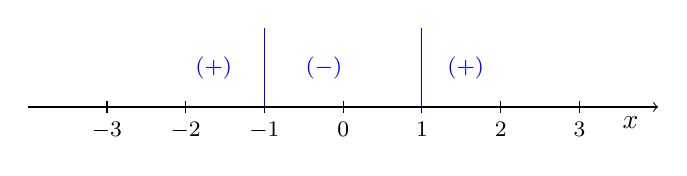
\begin{tikzpicture}
			
			% Gitternetzlinien
			%\draw[xstep=1cm, ystep=1cm, very thin, color=lightgray] (-4,4) grid (4,-2);
			% x-Achse
			\draw[->] (-4,0) -- (4,0) node[below,xshift=-1em] {$x$}; 
			%Zahlen auf x-Achse
			\foreach \x in {-3,...,3}
			\draw[shift={(\x,0)},color=black] (0pt,2pt) -- (0pt,-2pt) node[below] {\footnotesize $\x$};
			
			%\draw[color=black] (0pt,-10pt) node[right] {\footnotesize $0$};
			
			\draw [color=blue] (-2,0.5) node[right] {\footnotesize $(+)$};;
			\draw [color=blue] (-0.60,0.5) node[right] {\footnotesize $(-)$};;
			\draw [color=blue] (1.2,.5) node[right] {\footnotesize $(+)$};;
			\draw [color=blue] (-1,0) -- (-1,1);
			\draw [color=blue] (1,0) -- (1,1);
			
			\end{tikzpicture}\\
		\end{center}
		
		Der Definitionsbereich für $ g(x)=\ln(\frac{x^2+1}{x^2-1}) $ ist:\\
		\begin{align*}
		\mathbb{D}_g= \; ]-\infty,-1[\;\;\cup \;\;]1,+\infty[
		\end{align*}
	\end{quote}
	zu (ii):\\
	\begin{quote}
		Bestimme $ x\in \mathbb{R} $ mit $ \frac{1}{x^2}>0 $\\
		Der Definitionsbereich für $h(x)=\frac{1}{x^2}$ ist:\\
		\begin{align*}
		\mathbb{D}_h=\mathbb{R}\setminus \{0\}\\
		\end{align*}	
	\end{quote}
\newpage
\noindent
	Der Definitionsbereich von $ f(x)=\ln\bigg(\frac{x^2+1}{x^2-1}\bigg)-\ln\bigg(\frac{1}{x^2}\bigg) $ ist nun die Schnittmenge von $ \mathbb{D}_g $ und $ \mathbb{D}_h $.\\
	\begin{align*}
	\mathbb{D}_f&=\mathbb{D}_g\cap\mathbb{D}_h\\
	&=\big(]-\infty,-1[\;\;\cup \;\;]1,+\infty[\big)\;\;\cap\;\;\mathbb{R}\setminus \{0\}\\
	\end{align*}
	Fazit:\\
	\begin{align*}
	\mathbb{D}_f&=]-\infty,-1[\;\;\cup \;\;]1,+\infty[
	\end{align*}
\end{quote}
\href{https://youtu.be/3Xab3Mt4204}{Video 20}\\
$ \blacktriangleright $ Ableitung von $ f(x)=\ln\bigg(\frac{x^2+1}{x^2-1}\bigg)-\ln\bigg(\frac{1}{x^2}\bigg) $\\
\begin{quote}
	\begin{align*}
	f'(x)&=\bigg (\ln\bigg(\frac{x^2+1}{x^2-1}\bigg)-\ln\bigg(\frac{1}{x^2}\bigg)\bigg)'\\
	&=\bigg(\ln\bigg(\frac{x^2+1}{x^2-1}\bigg)\bigg)'-\bigg(\ln\bigg(\frac{1}{x^2}\bigg)\bigg)'\;\;\text{\tiny Summenregel }\\
	\end{align*}
	NR.:\\
	\begin{align*}
	\bigg(\ln\bigg(\frac{x^2+1}{x^2-1}\bigg)\bigg)'&=\frac{1}{\frac{x^2+1}{x^2-1}}\cdot \bigg(\frac{x^2+1}{x^2-1}\bigg)'=\frac{x^2-1}{x^2+1}\cdot\frac{(x^2+1)'(x^2-1)-(x^2+1)(x^2-1)'}{(x^2-1)^2}\\
	&=\frac{x^2-1}{x^2+1}\cdot\frac{2x(x^2-1)-2x(x^2+1)}{(x^2-1)^2}\\
	&=\frac{x^2-1}{x^2+1}\cdot\frac{2x^3-2x-2x^3-2x}{(x^2-1)^2}=\frac{(x^2-1)(-4x)}{(x^2+1)(x^2-1)^2}\\
	&=\frac{-4x}{(x^2+1)(x^2-1)}=\frac{-4x}{x^4-1}
	\end{align*}
	Nun ergibt sich:\\
	\begin{align*}
	f'(x)&=\frac{-4x}{x^4-1}-\bigg(\ln\bigg(\frac{1}{x^2}\bigg)\bigg)'\\
	&=\frac{-4x}{x^4-1}-\frac{1}{\frac{1}{x^2}}\cdot\bigg(\frac{1}{x^2}\bigg)'\;\;\text{\tiny NR.: $\bigg(\frac{1}{x^2}\bigg)'=\frac{-2}{x^3} $}\\
	&=\frac{-4x}{x^4-1}-\frac{1}{\frac{1}{x^2}}\cdot\bigg(\frac{-2}{x^3}\bigg)=\frac{-4x}{x^4-1}-x^2\bigg(\frac{-2}{x^3}\bigg)\\
	&=\frac{-4x}{x^4-1}+\frac{2}{x}
	\end{align*}
\end{quote}
\subsection{Das notwendige Kriterium für Extrema}
\href{https://youtu.be/IkfZZjapfWk}{Video 21}\\
Sei $ f: I\longmapsto \mathbb{R} $ diffbar auf $ I\subseteq \mathbb{R} $ und $ x_0 $ ein innerer Punkt (kein Randpunkt vom Intervall $ [a,b] $).\\
Hat $ f  $ ein Maximum oder Minimum in $ x_0 $, dann gilt:\\
\begin{align*}
f'(x_0)=0
\end{align*}
Beispiel:\\
\textbullet\;\; $ f:\mathbb{R}\longmapsto[0,\infty[ $ mit $ x\longmapsto x^2 $\\
\begin{quote}
	\begin{center}
		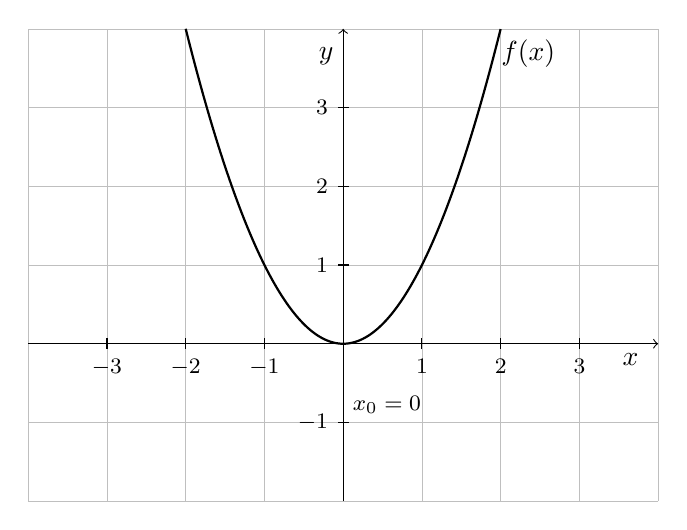
\begin{tikzpicture}
		
		% Gitternetzlinien
		\draw[xstep=1cm, ystep=1cm, very thin, color=lightgray] (-4,4) grid (4,-2);
		% x-Achse
		\draw[->] (-4,0) -- (4,0) node[below,xshift=-1em] {$x$}; 
		%Zahlen auf x-Achse
		\foreach \x in {-3,...,-1}
		\draw[shift={(\x,0)},color=black] (0pt,2pt) -- (0pt,-2pt) node[below] {\footnotesize $\x$};
		\foreach \x in {1,...,3}
		\draw[shift={(\x,0)},color=black] (0pt,2pt) -- (0pt,-2pt) node[below] {\footnotesize $\x$};
		% y-Achse 
		\draw[->] (0,-2) -- (0,4) node[left,yshift=-1em] {$y$};%node[above left]
		%Zahlen auf y-Achse
		\foreach \y in {-1,...,-1}
		\draw[shift={(0,\y)},color=black] (2pt,0pt) -- (-2pt,0pt) node[left] {\footnotesize $\y$};
		\foreach \y in {1,...,3}
		\draw[shift={(0,\y)},color=black] (2pt,0pt) -- (-2pt,0pt) node[left] {\footnotesize $\y$};
		%Ursprung
		\draw[color=black] (0pt,-22pt) node[right] {\footnotesize $x_0=0$};
		
		%\draw[thick,color=black] plot[samples=200, domain=2:4] 
		%(\x,{2}) node[below, xshift=-5em] {$h(x)$};
		
		\draw[thick,color=black] plot[samples=200, domain=-2:2] 
		(\x,{\x*\x}) node[below, xshift=1em]{$f(x)$};
		
		
		
		\end{tikzpicture}\\
	\end{center}
	Es gilt:\\
	\begin{align*}
	f'(x_0)=f'(0)=2x=2\cdot 0=0\\
	\end{align*}
	Warum muß hier bei $ x_0=0 $ die Ableitung Null sein?\\
	\begin{center}
		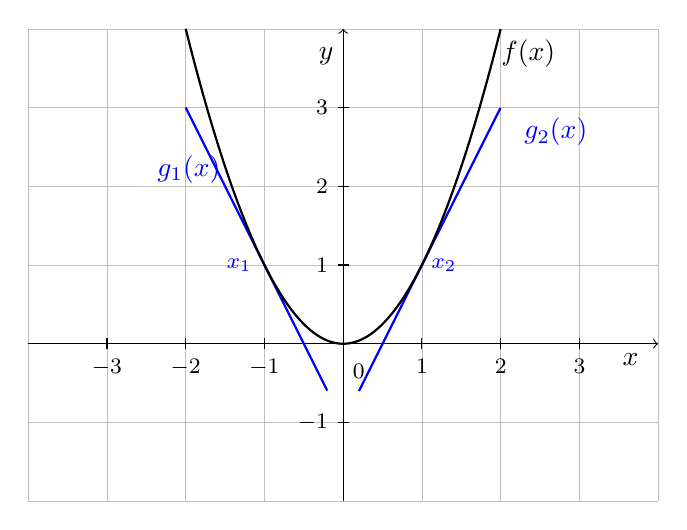
\begin{tikzpicture}
		
		% Gitternetzlinien
		\draw[xstep=1cm, ystep=1cm, very thin, color=lightgray] (-4,4) grid (4,-2);
		% x-Achse
		\draw[->] (-4,0) -- (4,0) node[below,xshift=-1em] {$x$}; 
		%Zahlen auf x-Achse
		\foreach \x in {-3,...,-1}
		\draw[shift={(\x,0)},color=black] (0pt,2pt) -- (0pt,-2pt) node[below] {\footnotesize $\x$};
		\foreach \x in {1,...,3}
		\draw[shift={(\x,0)},color=black] (0pt,2pt) -- (0pt,-2pt) node[below] {\footnotesize $\x$};
		% y-Achse 
		\draw[->] (0,-2) -- (0,4) node[left,yshift=-1em] {$y$};%node[above left]
		%Zahlen auf y-Achse
		\foreach \y in {-1,...,-1}
		\draw[shift={(0,\y)},color=black] (2pt,0pt) -- (-2pt,0pt) node[left] {\footnotesize $\y$};
		\foreach \y in {1,...,3}
		\draw[shift={(0,\y)},color=black] (2pt,0pt) -- (-2pt,0pt) node[left] {\footnotesize $\y$};
		%Ursprung
		\draw[color=black] (0pt,-10pt) node[right] {\footnotesize $0$};
		\draw[color=blue] (-1.6,1) node[right] {\footnotesize $x_1$};
		\draw[color=blue] (1,1) node[right] {\footnotesize $x_2$};
		\draw[thick,color=blue] plot[samples=200, domain=0.2:2] 
		(\x,{\x*2-1}) node[below, xshift=2em] {$g_2(x)$};
		\draw[thick,color=blue] plot[samples=200, domain=-2:-0.2] 
		(\x,{-\x*2-1}) node[yshift=80, xshift=-5em] {$g_1(x)$};
		\draw[thick,color=black] plot[samples=200, domain=-2:2] 
		(\x,{\x*\x}) node[below, xshift=1em]{$f(x)$};
		
		
		
		\end{tikzpicture}\\
	\end{center}
	Die Steigung von $ g_1(x_1) $ und $ g_2(x_2) $ ist gleich der Ableitung von $ f'(x_1)=2x_1 $ oder $f'(x_2)=2x_2  $ und für $ x_1<0 $ ist die Steigung negativ und für $ x_2>0 $ ist die Steigung positiv, also muß die Steigung zwischen $ x_1 $ und $ x_2 $ einmal Null werden.\\
\end{quote}
\newpage
\noindent
\textbullet \;\;$ g:\mathbb{R}\longmapsto\mathbb{R} $ mit $ x\longmapsto x^3 $\\
\begin{quote}
	\begin{center}
		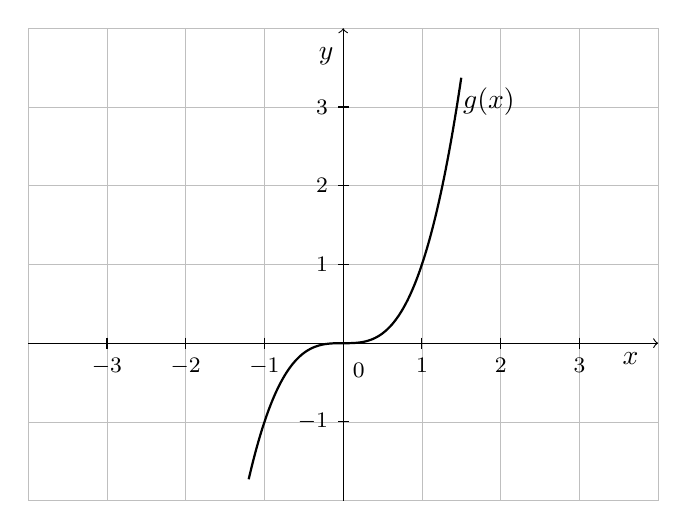
\begin{tikzpicture}
		
		% Gitternetzlinien
		\draw[xstep=1cm, ystep=1cm, very thin, color=lightgray] (-4,4) grid (4,-2);
		% x-Achse
		\draw[->] (-4,0) -- (4,0) node[below,xshift=-1em] {$x$}; 
		%Zahlen auf x-Achse
		\foreach \x in {-3,...,-1}
		\draw[shift={(\x,0)},color=black] (0pt,2pt) -- (0pt,-2pt) node[below] {\footnotesize $\x$};
		\foreach \x in {1,...,3}
		\draw[shift={(\x,0)},color=black] (0pt,2pt) -- (0pt,-2pt) node[below] {\footnotesize $\x$};
		% y-Achse 
		\draw[->] (0,-2) -- (0,4) node[left,yshift=-1em] {$y$};%node[above left]
		%Zahlen auf y-Achse
		\foreach \y in {-1,...,-1}
		\draw[shift={(0,\y)},color=black] (2pt,0pt) -- (-2pt,0pt) node[left] {\footnotesize $\y$};
		\foreach \y in {1,...,3}
		\draw[shift={(0,\y)},color=black] (2pt,0pt) -- (-2pt,0pt) node[left] {\footnotesize $\y$};
		%Ursprung
		\draw[color=black] (0pt,-10pt) node[right] {\footnotesize $0$};
		
		%\draw[thick,color=black] plot[samples=200, domain=-1.2:4] 
		%(\x,{2}) node[below, xshift=-5em] {$h(x)$};
		
		\draw[thick,color=black] plot[samples=200, domain=-1.2:1.5] 
		(\x,{\x*\x*\x }) node[below, xshift=1em]{$g(x)$};
		
		
		
		\end{tikzpicture}\\	
	\end{center}
	Es gilt:\\
	\begin{align*}
	g'(x_0)=3x^2_0=3\cdot 0^2=0\;\;\text{für }x_0=0\\
	\end{align*}
	$ g $ hat weder Maximum noch Minimum !\\
\end{quote}
Fazit: Die Umkehrung ist falsch. Die Aussage: Die Ableitung ist Null folgert nicht, dass hier ein Maximum oder Minimum ist.\\
\subsubsection{Das notwendige Kriterium für Extrema Aufgabe Teil I u. II}
\href{https://youtu.be/s-gd2f4tDws}{Video 22}\\
Bestimme alle globalen Extrema von der stetigen Funktion $ f:[-2,0]\longmapsto \mathbb{R} $ mit $ f(x)=\sqrt{x^3+x^2-2x} $.\\
Untersuche die inneren Punkten vom kompakten Intervall $x\in\; ]-2,0[  $ .\vspace*{4mm}\\
Berechne die Nullstellen von $ f'(x) $.\\
\begin{align*}
f'(x)=\bigg(\sqrt{x^3+x^2-2x}\bigg)'&=\frac{1}{2\sqrt{x^3+x^2-2x}}\cdot \bigg(x^3+x^2-2x\bigg)'\\
f'(x)&=\frac{3x^2+2x-2}{2\sqrt{x^3+x^2-2x}}\overset{!}{=} 0\\
\end{align*}
Bestimmung der Nullstellen vom Nenner. (Nenner darf nicht Null werden!)\\
\begin{align*}
x^3+x^2-2x=x(x^2+x-2)=x(x-1)(x+2)=0\\
\end{align*}
Die Nullstellen wären -2, 0 und 1, diese sind aber nicht im Intervall: $ \in \;]-2,0[  $ .\vspace*{4mm}\\
Bestimmung der Nullstellen vom Zähler $3x^2+2x-2=0 $ mit der p-q-Formel.\\
\begin{align*}
&3x^2+2x-2=0\\
&\Leftrightarrow x^2+\frac{2}{3}x-\frac{2}{3}x=0\\
\end{align*}
\begin{align*}
x_{1,2}&=-\frac{p}{2}\pm \sqrt{\bigg(\frac{p}{2}\bigg)^2-q}\\
&p=\frac{2}{3}\\
&q=\frac{-2}{3}\\
x_{1,2}&=-\frac{2}{3\cdot 2}\pm\sqrt{\bigg(\frac{2}{3\cdot2}\bigg)^2-(\frac{-2}{3})}\\
&=-\frac{1}{3}\pm\sqrt{\frac{1}{9}+\frac{2}{3}}\\
&=-\frac{1}{3}\pm\sqrt{\frac{7}{9}}\\
&=-\frac{1}{3}\pm \frac{1}{3}\sqrt{7}\\
&=\frac{-1\pm \sqrt{7}}{3}\\
x_1&=\frac{-1- \sqrt{7}}{3}\\
x_2&=\frac{-1+ \sqrt{7}}{3}\\
\end{align*}
Da $ x_2 $ offensichtlich größer Null ist, ist $ x\notin [-2,0] $.\\Nr: $ \sqrt{7} $ ist zwischen $ \sqrt{4} $ und $\sqrt{9}$, also zwischen $ 2 $ und $ 3 \Rightarrow x_2>0 $\\
Fazit:\\
Die einzige potentielle Extremstelle aus dem kompakten Intervall von  $ ]-2,0[  $ ist  $x_1=\frac{-1- \sqrt{7}}{3}  $.\\
\href{https://youtu.be/RrEGA0egEKQ}{Video 23}\\
Randpunktuntersuchung bei $ x_3=-2 $ und $ x_4=0$\\
\begin{align*}
&f(x)=\sqrt{x^3+x^2-2x}=\sqrt{x(x^2+x-2)}=\sqrt{x(x-1)(x+2)}\\
&\Rightarrow\\
&f(x_3)=f(-2)=0\\
&f(x_4)=f(0)=0\\
\end{align*}
Für $ x_1=\frac{-1-\sqrt{7}}{3} $ gilt:\\
\begin{align*}
&f(x_1)=\sqrt{\underbrace {x_1}_{<0}\underbrace {(x_1-1)}_{<0}\underbrace {(x_1-2)}_{>0}}\\
&\Rightarrow\\
&f(x_1)=f\bigg(\frac{-1-\sqrt{7}}{3}\bigg)>0\\
\end{align*}
In $ x_3 $ und $ x_4 $ hat $ f $ ein globales Minimum, weil $ f(x_1)>0 $ ist.\\
In $ x_1 $ hat f ein Maximum.\\
\newpage
\noindent
Bemerkung:\\
Da $ f $ stetig auf einen kompakten Intevall ist nimmt  $ f $ ein Maximum und ein Minimun an.\\
\begin{center}
	$  f:[-2,0]\longmapsto \mathbb{R} $ mit $ f(x)=\sqrt{x^3+x^2-2x} $\\
	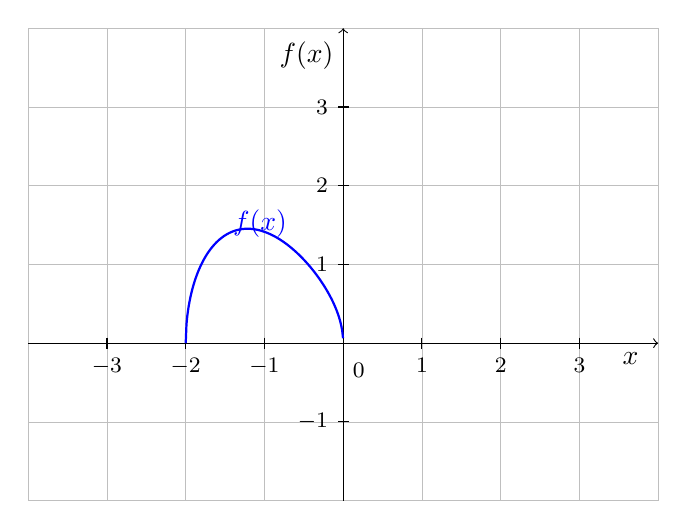
\begin{tikzpicture}
	
	% Gitternetzlinien
	\draw[xstep=1cm, ystep=1cm, very thin, color=lightgray] (-4,4) grid (4,-2);
	% x-Achse
	\draw[->] (-4,0) -- (4,0) node[below,xshift=-1em] {$x$}; 
	%Zahlen auf x-Achse
	\foreach \x in {-3,...,-1}
	\draw[shift={(\x,0)},color=black] (0pt,2pt) -- (0pt,-2pt) node[below] {\footnotesize $\x$};
	\foreach \x in {1,...,3}
	\draw[shift={(\x,0)},color=black] (0pt,2pt) -- (0pt,-2pt) node[below] {\footnotesize $\x$};
	% y-Achse 
	\draw[->] (0,-2) -- (0,4) node[left,yshift=-1em] {$f(x)$};%node[above left]
	%Zahlen auf y-Achse
	\foreach \y in {-1,...,-1}
	\draw[shift={(0,\y)},color=black] (2pt,0pt) -- (-2pt,0pt) node[left] {\footnotesize $\y$};
	\foreach \y in {1,...,3}
	\draw[shift={(0,\y)},color=black] (2pt,0pt) -- (-2pt,0pt) node[left] {\footnotesize $\y$};
	%Ursprung
	\draw[color=black] (0pt,-10pt) node[right] {\footnotesize $0$};
	
	
	
	\draw[thick,color=blue] plot[samples=200, domain=-2:0] 
	(\x,{sqrt(\x*\x*\x+\x*\x-2*\x)}) node[below, xshift=-3em,yshift=5em]{$f(x)$};
	
	
	
	\end{tikzpicture}\\
\end{center}
\subsection{Der Mittelwertsatz (der Differentialrechnung)}
\href{https://youtu.be/VGZF-dpPEDY}{Video 24}\\
Sei $ f: \mathbb{R}\supset \mathbb{I}\longmapsto \mathbb{R} $ diffbar auf dem Intevall $ I $ und $ a,b\in \mathbb{I} $ mit $ a\neq b $, dann existiert $ x_0 $ zwischen $ a $ und $ b $ mit:\\
\begin{align*}
f'(x_0)=\frac{f(b)-f(a)}{b-a}\\
\end{align*}
\begin{center}
	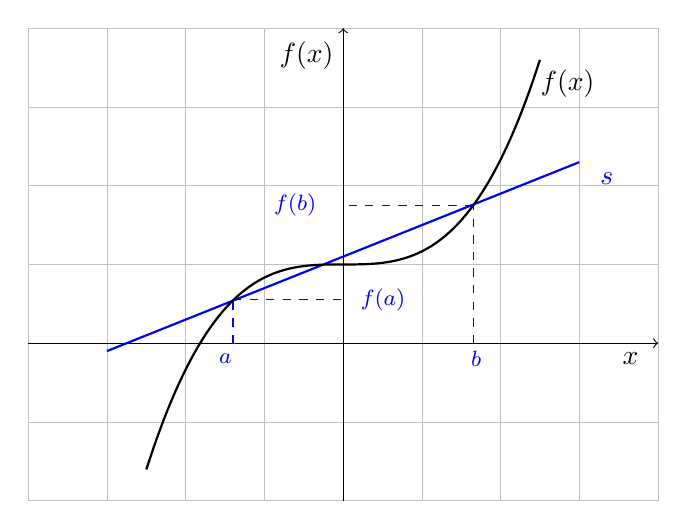
\begin{tikzpicture}
	
	% Gitternetzlinien
	\draw[xstep=1cm, ystep=1cm, very thin, color=lightgray] (-4,4) grid (4,-2);
	% x-Achse
	\draw[->] (-4,0) -- (4,0) node[below,xshift=-1em] {$x$}; 
	%Zahlen auf x-Achse
	%\foreach \x in {-3,...,-1}
	%\draw[shift={(\x,0)},color=black] (0pt,2pt) -- (0pt,-2pt) node[below] {\footnotesize $\x$};
	%\foreach \x in {1,...,3}
	%\draw[shift={(\x,0)},color=black] (0pt,2pt) -- (0pt,-2pt) node[below] {\footnotesize $\x$};
	% y-Achse 
	\draw[->] (0,-2) -- (0,4) node[left,yshift=-1em] {$f(x)$};%node[above left]
	%Zahlen auf y-Achse
	%\foreach \y in {-1,...,-1}
	%\draw[shift={(0,\y)},color=black] (2pt,0pt) -- (-2pt,0pt) node[left] {\footnotesize $\y$};
	%\foreach \y in {1,...,3}
	%\draw[shift={(0,\y)},color=black] (2pt,0pt) -- (-2pt,0pt) node[left] {\footnotesize $\y$};
	%Ursprung
	\draw[color=blue] (1.5,-0.2) node[right] {\footnotesize $b$};
	\draw[color=blue] (-1,1.75) node[right] {\footnotesize $f(b)$};
	\draw[color=blue,dashed] (1.65,0)--(1.65,1.75);
	\draw[color=blue,dashed] (1.65,1.75)--(0,1.75);
	
	
	
	\draw[color=blue] (-1.7,-0.2) node[right] {\footnotesize $a$};
	\draw[color=blue] (0.1,0.55) node[right] {\footnotesize $f(a)$};
	\draw[color=blue,dashed] (-1.4,0)--(-1.4,0.6);
	\draw[color=blue,dashed] (-1.4,0.55)--(0,0.55);
	\draw[thick,color=blue] plot[samples=200, domain=-3:3] 
	(\x,{0.4*\x+1.1}) node[below, xshift=1em]{$s$};
	\draw[thick,color=black] plot[samples=200, domain=-2.5:2.5] 
	(\x,{\x*\x*\x/6+1}) node[below, xshift=1em]{$f(x)$};
	
	
	
	\end{tikzpicture}\\
\end{center}
Die Formel der Sekante $ s $ ist :\\
\begin{align*}
&s(x)=f(a)+\frac{f(b)-f(a)}{b-a}(x-a)\;\;\text{\tiny Herleitung: siehe Kapitel 8.1} \\
&\Rightarrow \text{die Steigung der Geraden ist: }\;\;\frac{f(b)-f(a)}{b-a}
\end{align*}
Also existiert mindestens eine Steigung von $ f(x_0) $ mit $ m=\frac{f(b)-f(a)}{b-a} $ zwischen $ a $ und $ b $.\\
Eine Parallelverschiebung von $ s(x) $ ergibt $ g(x_0)$ mit der Steigung $ f'(x_0) $.\\
\begin{center}
	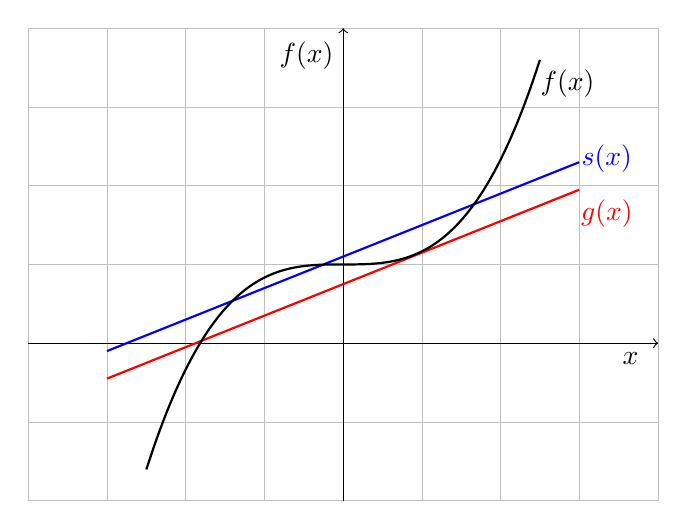
\begin{tikzpicture}
	
	% Gitternetzlinien
	\draw[xstep=1cm, ystep=1cm, very thin, color=lightgray] (-4,4) grid (4,-2);
	% x-Achse
	\draw[->] (-4,0) -- (4,0) node[below,xshift=-1em] {$x$}; 
	%Zahlen auf x-Achse
	%\foreach \x in {-3,...,-1}
	%\draw[shift={(\x,0)},color=black] (0pt,2pt) -- (0pt,-2pt) node[below] {\footnotesize $\x$};
	%\foreach \x in {1,...,3}
	%\draw[shift={(\x,0)},color=black] (0pt,2pt) -- (0pt,-2pt) node[below] {\footnotesize $\x$};
	% y-Achse 
	\draw[->] (0,-2) -- (0,4) node[left,yshift=-1em] {$f(x)$};%node[above left]
	%Zahlen auf y-Achse
	%\foreach \y in {-1,...,-1}
	%\draw[shift={(0,\y)},color=black] (2pt,0pt) -- (-2pt,0pt) node[left] {\footnotesize $\y$};
	%\foreach \y in {1,...,3}
	%\draw[shift={(0,\y)},color=black] (2pt,0pt) -- (-2pt,0pt) node[left] {\footnotesize $\y$};
	%Ursprung
	
	\draw[thick,color=red] plot[samples=200, domain=-3:3] 
	(\x,{0.4*\x+0.75}) node[below, xshift=1em,yshift=0em]{$g(x)$};
	
	
	\draw[thick,color=blue] plot[samples=200, domain=-3:3] 
	(\x,{0.4*\x+1.1}) node[below, xshift=1em,yshift=1em]{$s(x)$};
	\draw[thick,color=black] plot[samples=200, domain=-2.5:2.5] 
	(\x,{\x*\x*\x/6+1}) node[below, xshift=1em]{$f(x)$};
	
	
	
	\end{tikzpicture}\\
\end{center}
\underline{Der Satz von Rolle}\\
Wenn gilt:\\
\begin{align*}
f(a)=f(b)\\
\end{align*}
Dann existiert ein $ x_0 $ zwischen $ a $ und $ b $ mit:\\
\begin{align*}
f'(x_0)=0\\
\end{align*}
\begin{center}
	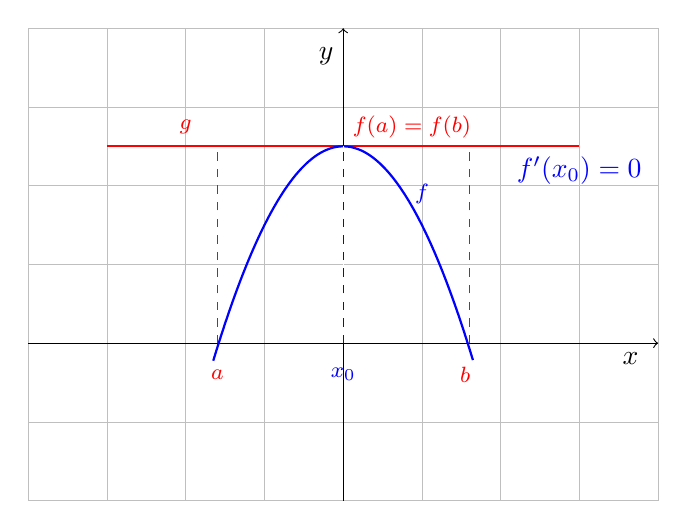
\begin{tikzpicture}
	
	% Gitternetzlinien
	\draw[xstep=1cm, ystep=1cm, very thin, color=lightgray] (-4,4) grid (4,-2);
	% x-Achse
	\draw[->] (-4,0) -- (4,0) node[below,xshift=-1em] {$x$}; 
	%Zahlen auf x-Achse
	%\foreach \x in {-3,...,-1}
	%\draw[shift={(\x,0)},color=black] (0pt,2pt) -- (0pt,-2pt) node[below] {\footnotesize $\x$};
	%\foreach \x in {1,...,3}
	%\draw[shift={(\x,0)},color=black] (0pt,2pt) -- (0pt,-2pt) node[below] {\footnotesize $\x$};
	% y-Achse 
	\draw[->] (0,-2) -- (0,4) node[left,yshift=-1em] {$y$};%node[above left]
	%Zahlen auf y-Achse
	%\foreach \y in {-1,...,-1}
	%\draw[shift={(0,\y)},color=black] (2pt,0pt) -- (-2pt,0pt) node[left] {\footnotesize $\y$};
	%\foreach \y in {1,...,3}
	%\draw[shift={(0,\y)},color=black] (2pt,0pt) -- (-2pt,0pt) node[left] {\footnotesize $\y$};
	%Ursprung
	
	\draw[thick,color=red] plot[samples=200, domain=-3:3] 
	(\x,{2.5}) node[below,color=blue,yshift=0em]{$f'(x_0)=0$};
	
	\draw[color=blue] (0,-0.4) node {\footnotesize $x_0$};
	
	\draw[thick,color=blue] plot[samples=200, domain=-1.65:1.65] 
	(\x,{-\x*\x+2.5});
	\draw[color=red] (0,2.75) node[right] {\footnotesize $f(a)=f(b)$};
	\draw[color=red] (-1.8,-0.4) node[right] {\footnotesize $a$};
	\draw[color=red,dashed] (-1.6,0)--(-1.6,2.5);
	\draw[color=red] (1.36,-0.4) node[right,] {\footnotesize $b$};
	\draw[color=red,dashed] (1.6,0)--(1.6,2.5);
	\draw[color=white] (0,0)--(0,2.5);
	\draw[color=blue,dashed] (0,0)--(-0,2.5);
	\draw[color=blue] (1,1.9) node {\footnotesize $f$};
	\draw[color=red] (-2,2.75) node {\footnotesize $g$};
	\end{tikzpicture}\\
\end{center}
\subsubsection{Aufgabe 1 zum Mittelwertsatz}
\href{https://youtu.be/EaH9h63wHm0}{Video 25}\\
Zeige mit dem MWS, dass für $ x\geq 0: \ln(2x+1)\leq 2x $ gilt:\\
Betrachte die Funktion: $ f(x)=\ln(2x+1) $ und wende hier den MWS an und versuche durch Umformung und Abschätzung der Gleichung die Ungleichung zu beweisen.\\\\
\begin{align*}
f(x)&=\ln(2x+1)\\
f'(x)&=\frac{2}{2x+1}\\
\end{align*}
Wählt man $ a=0 $ und $ x>0 $, dann existiert nach MWS ein $ x_0 $ zwischen $ a $ und $ x $ mit:\\
\begin{align*}
&f'(x_0)=\frac{f(x)-f(a)}{x-a}\\
&\Leftrightarrow\\
&\big(\ln(2x+1)\big)'_{(x_0)}=\frac{\ln(2x+1)-\ln(1)}{x}\\
&\Leftrightarrow\\
&\frac{2}{2x_0+1}=\frac{\ln(2x+1)}{x}\\
\end{align*}
Nun gilt, für $ x_0>0 $ und durch Abschätzung von $ 2x_0+1 $:\\
\begin{align*}
&2x_0+1>1\;\;\text{für }\;x_0>0\\
&\Rightarrow\\
&\frac{2}{2x_0+1}<2\\
\end{align*}
Dann gilt für $ x>0 $:\\
\begin{align*}
&\frac{\ln(2x+1)}{x}=\frac{2}{2x_0+1}<2\\
&\Rightarrow\\
&\frac{\ln(2x+1)}{x}<2\;\;|\text{\tiny $\cdot x$ }\\
&\ln(2x+1)<2x
\end{align*}
Für $ x=0 $ gilt:\\
\begin{align*}
\ln(2x+1)&\leq 2x\\
\ln(2\cdot0+1)&\leq 2\cdot 0\\
0&=0
\end{align*}
Nun gilt für $ x\geq0 $:\\
\begin{align*}
\ln(2x+1)\leq 2x_{_{\Square}}\\
\end{align*}
\subsubsection{Aufgabe 2 zum Mittelwertsatz}
\href{https://youtu.be/uzNiQL4wJ-M}{Video 26}\\
Zeige mit dem MWS, dass für alle $ x\geq 0 $ gilt $ \sqrt{1+2x}\leq 1+x $\\
Für $ x=0 $ gilt:\\
\begin{align*}
\sqrt{1+2x}&\leq 1+x\\
\sqrt{1+2\cdot 0}&\leq 1+0\\
1&=1\\
\end{align*}
Betrachte nun nur die linke Seite der Ungleichung und wende dann den MWS an.\\
\begin{align*}
f(x)&=\sqrt{1+2x}\\
f'(x)&=\frac{1}{2\sqrt{1+2x}}\cdot \big(1+2x\big)'=\frac{1}{\sqrt{1+2x}}\\
\end{align*}
Wähle $ a=0 $ und $ x>0 $.\\
Dann existiert ein $ x_0 $ zwischen $ a $ und $ x $ mit:\\
\begin{align*}
f'(x_0)=\frac{f(x)-f(a)}{x-a}\\
\end{align*}
Dann gilt mit $ x_0 $ und $ a=0 $ :\\
\begin{align*}
\frac{1}{\sqrt{1+2x_0}}=\frac{\sqrt{1+2x}-\sqrt{1-0}}{x-0}=\frac{\sqrt{1+2x}-1}{x}\\
\end{align*}
Nun wird $ \frac{1}{\sqrt{1+2x_0}} $ abgeschätzt.\\
Es gilt für $ x_0>0 $\\
\begin{align*}
&\sqrt{1+2x_0}>1\\
&\Leftrightarrow\\
&\frac{1}{\sqrt{1+2x_0}}<1\\
\end{align*}
Dann gilt für $ x>0 $:\\
\begin{align*}
1&>\frac{1}{\sqrt{1+2x_0}}=\frac{\sqrt{1+2x}-1}{x}\\
&\Rightarrow\\
1&>\frac{\sqrt{1+2x}-1}{x}\\
1&>\frac{\sqrt{1+2x}}{x}-\frac{1}{x}\;\;|\text{\tiny $ +\frac{1}{x} $ }\\
1+\frac{1}{x}&>\frac{\sqrt{1+2x}}{x}-\frac{1}{x}+\frac{1}{x}\;\;|\text{\tiny $ \cdot x $ }\\
1+x&>\sqrt{1+2x}\\
\end{align*}
Nun gilt für $ x\geq  0 $ :\\
\begin{align*}
\sqrt{1+2x}\leq 1+x_{_{\Square}}
\end{align*}
\subsection{Folgerung des Mittelwertsatzes}
\subsubsection{Monotonoie von Folgen}
\href{https://youtu.be/M2WZh7_cc0s}{Video 27}\\
Eine Funktion $ f:\mathbb{R}\supseteq \mathbb{D}_f\longmapsto \mathbb{W}_f\subseteq\mathbb{R} $ heißt monoton steigend, wenn für alle $ a,b\in \mathbb{D}_f $ mit $ a<b $ folgt $ f(a)\leq f(b) $.\\
Analog definieren wir monoton fallend, wenn für alle $ a,b\in \mathbb{D}_f $ mit $ a<b $ folgt $ f(a)\geq f(b) $.\\
\begin{center}
	
	
	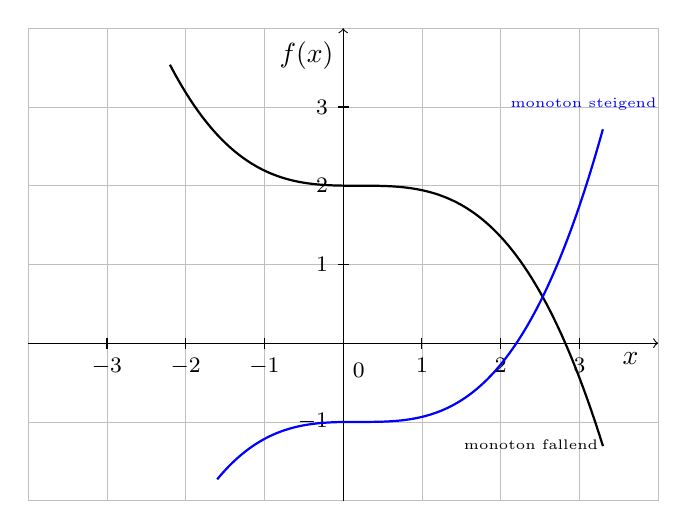
\begin{tikzpicture}
	
	% Gitternetzlinien
	\draw[xstep=1cm, ystep=1cm, very thin, color=lightgray] (-4,4) grid (4,-2);
	% x-Achse
	\draw[->] (-4,0) -- (4,0) node[below,xshift=-1em] {$x$}; 
	%Zahlen auf x-Achse
	\foreach \x in {-3,...,-1}
	\draw[shift={(\x,0)},color=black] (0pt,2pt) -- (0pt,-2pt) node[below] {\footnotesize $\x$};
	\foreach \x in {1,...,3}
	\draw[shift={(\x,0)},color=black] (0pt,2pt) -- (0pt,-2pt) node[below] {\footnotesize $\x$};
	% y-Achse 
	\draw[->] (0,-2) -- (0,4) node[left,yshift=-1em] {$f(x)$};%node[above left]
	%Zahlen auf y-Achse
	\foreach \y in {-1,...,-1}
	\draw[shift={(0,\y)},color=black] (2pt,0pt) -- (-2pt,0pt) node[left] {\footnotesize $\y$};
	\foreach \y in {1,...,3}
	\draw[shift={(0,\y)},color=black] (2pt,0pt) -- (-2pt,0pt) node[left] {\footnotesize $\y$};
	%Ursprung
	\draw[color=black] (0pt,-10pt) node[right] {\footnotesize $0$};
	
	\draw[thick,color=black] plot[samples=200, domain=-2.2:3.3] 
	(\x,{-(\x-0.2)^3/9+2.0}) node[below, xshift=-2.6em,yshift=0.6em] {\tiny monoton fallend};
	
	\draw[thick,color=blue] plot[samples=200, domain=-1.6:3.3] 
	(\x,{(\x-0.2)^3/8-1}) node[below, xshift=-0.7em,yshift=1.5em]{\footnotesize \tiny monoton steigend};
	
	
	
	\end{tikzpicture}\\
\end{center}
Bei streng monoton gilt:\\
\begin{align*}
f(a)<f(b)\\
f(a)>f(b)\\
\end{align*}
\begin{center}
	
	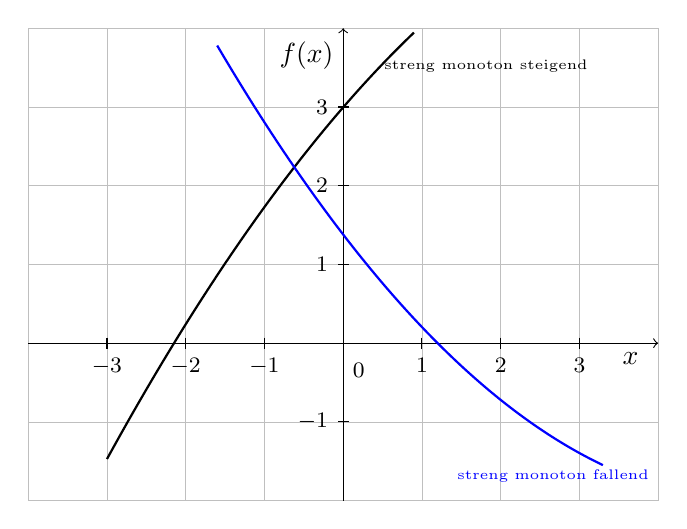
\begin{tikzpicture}
	
	% Gitternetzlinien
	\draw[xstep=1cm, ystep=1cm, very thin, color=lightgray] (-4,4) grid (4,-2);
	% x-Achse
	\draw[->] (-4,0) -- (4,0) node[below,xshift=-1em] {$x$}; 
	%Zahlen auf x-Achse
	\foreach \x in {-3,...,-1}
	\draw[shift={(\x,0)},color=black] (0pt,2pt) -- (0pt,-2pt) node[below] {\footnotesize $\x$};
	\foreach \x in {1,...,3}
	\draw[shift={(\x,0)},color=black] (0pt,2pt) -- (0pt,-2pt) node[below] {\footnotesize $\x$};
	% y-Achse 
	\draw[->] (0,-2) -- (0,4) node[left,yshift=-1em] {$f(x)$};%node[above left]
	%Zahlen auf y-Achse
	\foreach \y in {-1,...,-1}
	\draw[shift={(0,\y)},color=black] (2pt,0pt) -- (-2pt,0pt) node[left] {\footnotesize $\y$};
	\foreach \y in {1,...,3}
	\draw[shift={(0,\y)},color=black] (2pt,0pt) -- (-2pt,0pt) node[left] {\footnotesize $\y$};
	%Ursprung
	\draw[color=black] (0pt,-10pt) node[right] {\footnotesize $0$};
	
	\draw[thick,color=black] plot[samples=200, domain=-3:0.9] 
	(\x,{-(\x-5.2)^2/9+6.0}) node[below, xshift=2.6em,yshift=-0.6em] {\tiny streng monoton steigend};
	
	\draw[thick,color=blue] plot[samples=200, domain=-1.6:3.3] 
	(\x,{(\x-5.2)^2/8-2}) node[below, xshift=-1.8em,yshift=0.2em]{\footnotesize \tiny streng monoton fallend};
	
	
	
	\end{tikzpicture}\\
\end{center}
Beispiel:\\
Zeige, dass $ f:\mathbb{R}\longmapsto \mathbb{R} $ mit $ f(x)=2x $ streng monoton steigend ist.\\
Beweis:\\
Seien $ a,b\in \mathbb{R} $ und $ a<b $\\
Zu zeigen:\\
\begin{align*}
&f(a)<f(b)\\
&a<b\Rightarrow f(a)=2a<2b=f(b)_{_{\Square}}\\
\end{align*}
\paragraph{Monotonie von Funktionen Aufgabe 1}$  $\vspace*{3mm}\\
\href{https://youtu.be/BN9OWtPFY7g}{Video 28}\\
Zeige, dass die Funktion $ f:\;]0,\infty[ \;\longmapsto \mathbb{R}$ mit $ f(x) =\frac{1}{x}$ streng monoton fallend ist.\vspace*{4mm}\\
Für $ a,b\in \left] 0,\infty\right]  $ beliebig und mit $ a<b $ ist z.z. $ f(a)>f(b) $.\\
Beweis:\\
\begin{align*}
&a<b\\
&\Leftrightarrow\\
&\frac{1}{a}>\frac{1}{b}\\
&\Leftrightarrow\\
&f(b)=\frac{1}{b}<\frac{1}{a}=f(a)_{_{\Square}}\\
\end{align*}
Berachten wir $ \overset{\AC}{f}:\mathbb{R}\backslash \{0\}\longmapsto \mathbb{R}  $ mit $ f(x)=\frac{1}{x} $.
Diese Funktion ist nicht monoton!\\
Beweis:\\
Für $ a=-1 $ und $ b=1 $ gilt:\\
\begin{align*}
&a=-1<b=1\\
&\Leftrightarrow\\
&f(a)=-1<f(b)=1\Rightarrow  \text{monoton steigend }\\
\end{align*}
\begin{center}
	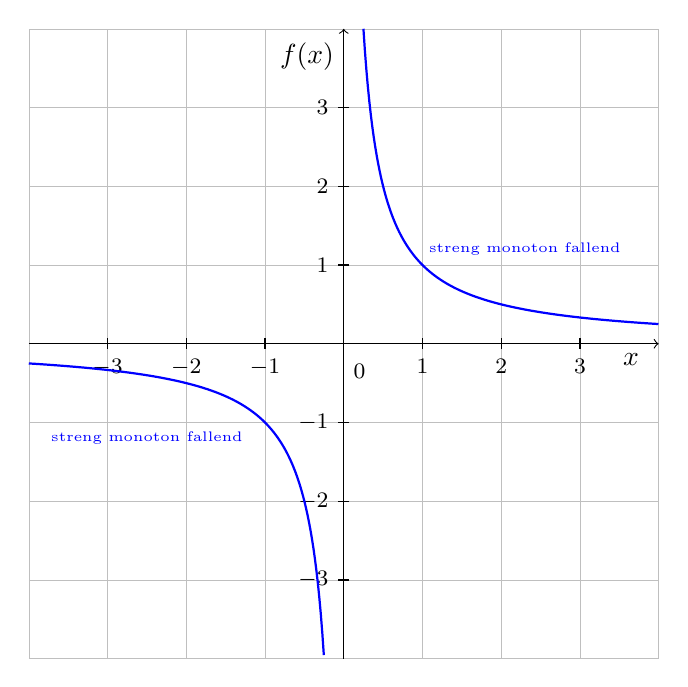
\begin{tikzpicture}
	
	% Gitternetzlinien
	\draw[xstep=1cm, ystep=1cm, very thin, color=lightgray] (-4,4) grid (4,-4);
	% x-Achse
	\draw[->] (-4,0) -- (4,0) node[below,xshift=-1em] {$x$}; 
	%Zahlen auf x-Achse
	\foreach \x in {-3,...,-1}
	\draw[shift={(\x,0)},color=black] (0pt,2pt) -- (0pt,-2pt) node[below] {\footnotesize $\x$};
	\foreach \x in {1,...,3}
	\draw[shift={(\x,0)},color=black] (0pt,2pt) -- (0pt,-2pt) node[below] {\footnotesize $\x$};
	% y-Achse 
	\draw[->] (0,-4) -- (0,4) node[left,yshift=-1em] {$f(x)$};%node[above left]
	%Zahlen auf y-Achse
	\foreach \y in {-1,...,-3}
	\draw[shift={(0,\y)},color=black] (2pt,0pt) -- (-2pt,0pt) node[left] {\footnotesize $\y$};
	\foreach \y in {1,...,3}
	\draw[shift={(0,\y)},color=black] (2pt,0pt) -- (-2pt,0pt) node[left] {\footnotesize $\y$};
	%Ursprung
	\draw[color=black] (0pt,-10pt) node[right] {\footnotesize $0$};
	
	\draw[thick,color=blue] plot[samples=200, domain=-4:-0.25] 
	(\x,{1/\x});% node[below, xshift=-5em] {$h(x)$};
	
	\draw[thick,color=blue] plot[samples=200, domain=0.25:4] 
	(\x,{1/\x});% node[below, xshift=1em]{$g(x)$};
	
	\draw[color=blue] (-2.5,-1.2) node {\tiny streng monoton fallend};
	\draw[color=blue] (2.3,1.2) node {\tiny streng monoton fallend};
	\end{tikzpicture}\\	
\end{center}
\paragraph{Monotonie von Funktionen Aufgabe 2}$  $\vspace*{3mm}\\
\href{https://youtu.be/EiJkuy1dVWc}{Video 29}\\
Zeige, dass die Funktion $ f:[0,\infty [\;  \longmapsto \;[0,\infty [  $ mit $ f(x)=\sqrt{x} $ streng monoton steigend ist.\vspace*{4mm}\\
Für $ a,b\in [0,\infty[$ beliebig, mit $ a<b $ ist z.z. $ f(a)<f(b) $\\
Beweis:
\begin{align*}
a<b\Leftrightarrow \frac{a}{b}<1\Leftrightarrow \sqrt{\frac{a}{b}}<1\Leftrightarrow \frac{\sqrt{a}}{\sqrt{b}}<1\Leftrightarrow \sqrt{a}<\sqrt{b}_{_{\Square}}\\
\end{align*}
Bemerkung (b kann nicht Null werden): \\
Da $a,b\in [0,\infty[ $ und $ a<b   \Rightarrow a=0\Rightarrow b>0$\\
\\
Also ist $ f(x)=\sqrt{x} $ streng monoton steigend.\\
\begin{center}
	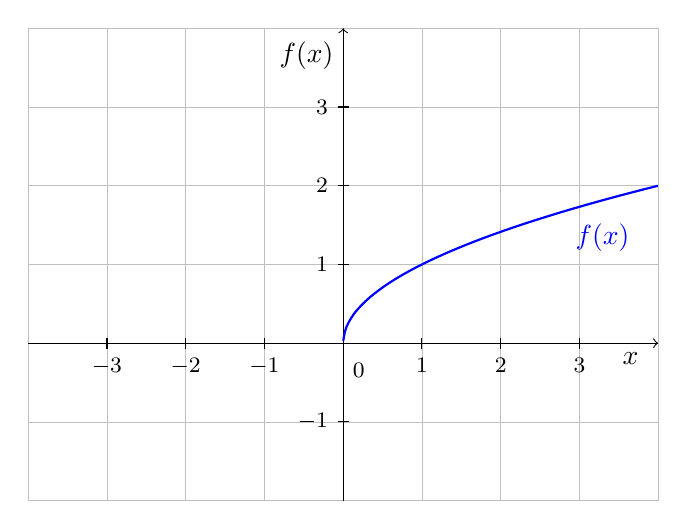
\begin{tikzpicture}
	
	% Gitternetzlinien
	\draw[xstep=1cm, ystep=1cm, very thin, color=lightgray] (-4,4) grid (4,-2);
	% x-Achse
	\draw[->] (-4,0) -- (4,0) node[below,xshift=-1em] {$x$}; 
	%Zahlen auf x-Achse
	\foreach \x in {-3,...,-1}
	\draw[shift={(\x,0)},color=black] (0pt,2pt) -- (0pt,-2pt) node[below] {\footnotesize $\x$};
	\foreach \x in {1,...,3}
	\draw[shift={(\x,0)},color=black] (0pt,2pt) -- (0pt,-2pt) node[below] {\footnotesize $\x$};
	% y-Achse 
	\draw[->] (0,-2) -- (0,4) node[left,yshift=-1em] {$f(x)$};%node[above left]
	%Zahlen auf y-Achse
	\foreach \y in {-1,...,-1}
	\draw[shift={(0,\y)},color=black] (2pt,0pt) -- (-2pt,0pt) node[left] {\footnotesize $\y$};
	\foreach \y in {1,...,3}
	\draw[shift={(0,\y)},color=black] (2pt,0pt) -- (-2pt,0pt) node[left] {\footnotesize $\y$};
	%Ursprung
	\draw[color=black] (0pt,-10pt) node[right] {\footnotesize $0$};
	
	
	
	\draw[thick,color=blue] plot[samples=200, domain=0.001:4] 
	(\x,{(\x)^0.5}) node[below, xshift=-2em,yshift=-1em]{$f(x)$};
	
	
	
	\end{tikzpicture}\\
\end{center}
\subsubsection{Monotoniekriterium}
\href{https://youtu.be/K_BfNKGb46I}{Video 30}\\
Sei $ f: \mathbb{I}\longmapsto \mathbb{R} $ differenzierbar auf dem Intervall $ \mathbb{I} $.\\
Für alle $ x\in \mathbb{I} $ gilt:\\
\begin{center}
	Monotoniekriterium\\
	\fbox{\parbox  {100mm} {
			1. $ f'(x)\geq 0 $, dann ist $ f $ auf $ \mathbb{I} $ monoton steigend.\\
			2. $ f'(x)> 0$, dann ist $ f $ auf $ \mathbb{I} $ streng monoton steigend.\\
			3. $ f'(x)\leq 0$, dann ist $ f $ auf $ \mathbb{I} $ monoton fallend.\\
			4. $ f'(x)< 0$, dann ist $ f $ auf $ \mathbb{I} $ streng monoton fallend.\\}}
\end{center}
Dies sind Folgerungen aus dem Mittelwertsatz.\\
Beweis zu 1.)\\
Sei $ f'(x)\geq 0 $ für alle $ x\in \mathbb{I} $.\\
Zz.: $ a,b\in \mathbb{I} $ und $ a<b\Rightarrow f(a)\leq f(b) $\\
Nach dem MWS existiert ein $ x_0 $ zwischen $ a $ und $ b $ mit $ f'(x)=\frac{f(b)-f(a)}{b-a} $\\
Mit der Vorraussetzung $ f'(x)\geq 0 $ gilt:\\
\begin{align*}
0&\leq f'(x)=\frac{f(b)-f(a)}{b-a} \\
0&\leq\frac{f(b)-f(a)}{b-a} \;\;|\text{\tiny $ \cdot (b-a) $ }\\
&\leq\frac{f(b)-f(a)(b-a)}{(b-a)} \\
&\leq f(b)-f(a)\\
&\Leftrightarrow f(a)\leq f(b)_{_{\Square}}
\end{align*}
Beispiel:\\
\textbullet\;\; $ f:[0,\infty[\;\longmapsto \;[0,\infty[ $ mit $ f(x)=x^2 $ ist monoton wachsend,weil gilt:\\
\begin{align*}
f'(x)=2x\geq 0 \;\;\text{für }\;\;x\in [0,\infty[\\
\end{align*}
\textbullet\;\; $ g:\;]0,\infty[\;\longmapsto \;]0,\infty[ $ mit $ g(x)=x^2 $ ist streng monoton wachsend,weil gilt:\\
\begin{align*}
g'(x)=2x > 0 \;\;\text{für }\;\;x\in ]0,\infty[\\
\end{align*}
\paragraph{Aufgabe zum Monotoniekriterium}$   $\vspace*{3mm}\\
\href{https://youtu.be/E2T-2jXem2Y}{Video 31}\\
Sei $ f:\mathbb{R}\longmapsto \mathbb{R} $ mit $ f(x)=2x^3+3x^2-12x+1 $ gegeben\\
Bestimme die Bereiche auf denen $ f $ streng monoton ist.\vspace*{2mm}\\
Betrachte:\\
\begin{align*}
f'(x)=(2x^3+3x^2-12x+1)'=6x^2+6x-12=6(x^2+x-2)\\
\end{align*}
Die Nullstellen von $ f'(x) =6(x^2+x-2)$ sind $ -2 $ und $ 1 $ \\
\begin{align*}
f'(x)=6(x-1)(x+2)\\
\end{align*}
Bei den Nullstellen hat man ein Vorzeichenwechsel und dies zeigt den Wechsel zwischen  monoton steigend und fallend. Ist $ f $ streng monoton, dann darf $ f'(x) $ nicht Null werden.\vspace*{2mm}\\
Bei $ x=-3 $ ist $ f'(x)=6(-3-1)(-3+2)\Rightarrow $ positiv $ f'(x)>0 $\\
Bei $ x=0 $ ist $ f'(x)=6(0-1)(0+2)\Rightarrow $ negativ $ f'(x)<0 $\\
Bei $ x=3 $ ist $ f'(x)=6(3-1)(3+2)\Rightarrow $ positiv $ f'(x)>0 $\\
\begin{center}
	
	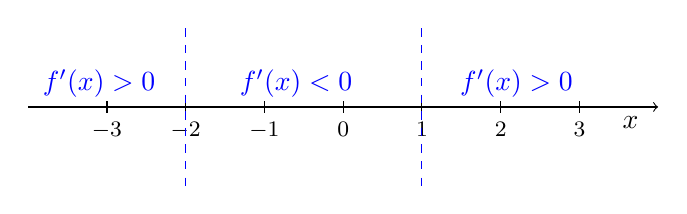
\begin{tikzpicture}
	
	
	% x-Achse
	\draw[->] (-4,0) -- (4,0) node[below,xshift=-1em] {$x$}; 
	%Zahlen auf x-Achse
	\foreach \x in {-3,...,3}
	\draw[shift={(\x,0)},color=black] (0pt,2pt) -- (0pt,-2pt) node[below] {\footnotesize $\x$};
	\draw [dashed,color=blue] (-2,1)--(-2,-1);
	\draw [dashed,color=blue] (1,1)--(1,-1);
	\draw [color=blue] (-3.1,0.3) node {$ f'(x)>0 $};
	\draw [color=blue] (2.2,0.3) node {$ f'(x)>0 $};
	\draw [color=blue] (-0.6,0.3) node {$ f'(x)<0 $};
	\end{tikzpicture}\\
\end{center}
Fazit:\\
(i)\;\,\,Für $ x\in \;]-\infty,-2[ $ ist $ f'(x) >0$\\
(ii) Für $ x\in \;]-2,1[ $ ist $ f'(x) <0$\\
(iii)\,Für $ x\in \;]1,\infty[ $ ist $ f'(x) >0$\vspace*{4mm}\\
$f(x) $ ist streng monoton steigend im Intervall:\\
\begin{align*}
x\in\;]-\infty,-2[\;\;\cup\;\;]1,\infty[\\
\end{align*}
$f(x) $ ist streng monoton fallend im Intervall:\\
\begin{align*}
x\in\;]-2,1[\\
\end{align*}
\subsubsection{Konstanzkriterium}
\href{https://youtu.be/SUuhqlbPbGI}{Video 32}\\
Sei $f:\mathbb{R}\supset \mathbb{I}\longmapsto \mathbb{R}$ auf $ \mathbb{I} $ diffbar.\\
Gelte $f'(x)=0$ für $x\in\mathbb{I}  $ dann ist $ f $ konstant, also von der Form $ f'(x)=0 $ für $ x\in \mathbb{I}, k\in\mathbb{R} $.\vspace*{2mm}\\
Nach dem MWS für alle $ a,b\in \mathbb{I} $ mit $ a\neq b $ existiert ein $ x_0 $ zwischen $ a $ und $ b $ mit $ f'(x)=\frac{f(b)-f(a)}{b-a} $.\vspace*{4mm}\\
Für $f$ konstant gilt dann:\\
\begin{align*}
&0=f'(x)=\frac{f(b)-f(a)}{b-a}\;\;|\text{\tiny $\cdot (b-a)$ } \\
&\Leftrightarrow f(b)-f(a)=0\\
&\Leftrightarrow f(b)=f(a)\\
\end{align*}
D.h. $ f(x)=k $ für alle $ x\in\mathbb{I} $ mit $ k\in \mathbb{R} $\vspace*{4mm}\\
Beispiel:\\
\textbullet\;\;Ist $ f $ konstant, dann gilt $ f'(x)=0 $ denn:\\
\begin{align*}
(f(x))'=(k)'=(k\cdot x^0)'=0\cdot k\cdot x^{-1}=0\\
\end{align*}
\textbullet\;\;$ f(x)=10\Rightarrow f'(x)=0 $ für alle $ x\in\mathbb{R} $\\
\begin{quote}
	Rückschluß nicht möglich, wenn $ f'(x)=10 $ erhält man nicht $ f(x) =10$!\\
\end{quote}
\paragraph{Aufgabe zum Konstanzkriterium}$  $\vspace*{3mm}\\
\href{https://youtu.be/mMXOmLVoRmo}{Video 33}\\
Bestimme alle diffbaren Funktionen $ f $ mit folgenden Eigenschaften:\\
(i)\; $ (f-p)'_{(x)}=0 $ für alle $ x\in \mathbb{R} $\\
(ii) $f(1)=p(1)$,
wobei $ p(x)=x^2+x-2 $ ist.\\
zu(i):\\
\begin{quote}
	Mit dem Konstanzkriterium folgt, dass $ f-p $ konstant ist:\\
	Es gilt:\\
	\begin{align*}
	&f(x)-p(x)=k\\
	&\Leftrightarrow f(x)=p(x)+k=x^2+x-2+k\\
	\end{align*}
\end{quote}
zu (ii):\\
\begin{quote}
	\begin{align*}
	f(1)=1^2+1-2+k=k=p(1)=0\Rightarrow k=0\\
	\end{align*}
\end{quote}
Dann sind alle diffbaren Funktionen mit den Eigenschften (i) und (ii) von der Form:\\
\begin{align*}
f(x)=x^2+x-2=p(x)\\
\end{align*}
\subsection{Regel von L’Hospital}
\href{https://youtu.be/wBqlghVLs04}{Video 34}\\
Seien $ f,g: \mathbb{I} \longmapsto \mathbb{R}$ diffbare Funktionen auf dem Intervall $\mathbb{I}\subset \mathbb{R}$ sowie $ x_0\in \mathbb{R}\cup \{\pm\infty\} $.\\
Es gelte weiterhin $ g'\neq 0 $ für alle $ x\in\mathbb{I}$ und es existiert der Limes\\
\begin{align*}
\lim\limits_ {x\to x_0} \frac{f'(x)}{g'(x)}=G\;\;\text{mit }\;\;  G\in \mathbb{R}\\
\end{align*}
dann folgt falls:\\
\textbullet \;\; $ \lim\limits_ {x\to x_0}f(x)= \lim\limits_ {x\to x_0}g(x)= 0 $\\
\begin{align*}
\lim\limits_ {x\to x_0} \frac{f'(x)}{g'(x)}=G
\end{align*}
\textbullet \;\; $ \lim\limits_ {x\to x_0}f(x)= \lim\limits_ {x\to x_0}g(x)= \pm\infty $\\
\begin{align*}
\lim\limits_ {x\to x_0} \frac{f'(x)}{g'(x)}=G
\end{align*}
Beispiel:\\
\begin{align*}
\lim\limits_ {x\to 0}\frac{\sin(x)}{x}\overset{L'H}{=}\lim\limits_ {x\to\ 0}\frac{(\sin(x))'}{(x)'}=\lim\limits_ {x\to 0} \frac{\cos(x)}{1}=\lim\limits_ {x\to 0} \cos(x)=1\\
\end{align*}
\subsubsection{Trick 1 zur Regel von L’Hospital}
\href{https://youtu.be/Chm62OX6xbE}{Video 35 }\\
Berechne falls existieren die folgenden Genzwerte.\\
(i)\;\;$ \lim\limits_ {x\to 0}\frac{\cos(x)-1}{x\cdot \sin(x)} $\\
(ii) $ \lim\limits_ {x\to 0}\frac{\ln(x+1)}{\ln(x-1)} $\vspace*{2mm}\\
Zu (i):\\
\begin{align*}
\lim\limits_ {x\to 0}\frac{\cos(x)-1}{x\cdot \sin(x)} \\
\end{align*}
Ist die Regel anwendbar?\\
\begin{align*}
\cos(0)-1&=0\\
0\cdot \sin(0)&=0\\
&\Rightarrow \frac{0}{0}\\
\end{align*}
\begin{align*}
\lim\limits_ {x\to 0}\frac{\cos(x)-1}{x\cdot \sin(x)}\overset{L'H}{=}\lim\limits_ {x\to 0}\frac{(\cos(x)-1)'}{(x\cdot \sin(x))'}=\lim\limits_ {x\to 0}\bigg[\frac{-\sin(x)}{\sin(x)+x\cdot \cos(x)}\bigg]
\end{align*}
\begin{align*}
-\sin(0)&=0\\
\sin(x)+x\cdot \cos(x)&=0\\
&\Rightarrow \frac{0}{0}\\
\end{align*}
Die Regel L'Hospital nochmals anwenden.\\
\begin{align*}
\lim\limits_ {x\to 0}\bigg[\frac{-\sin(x)}{\sin(x)+x\cdot \cos(x)}\bigg]\overset{L'H}{=}\lim\limits_ {x\to 0}\bigg[\frac{-\cos(x)}{\cos(x)+\cos(x)+x\cdot (-\sin(x))}\bigg]=\lim\limits_ {x\to 0}\bigg[\frac{-\cos(x)}{2\cdot \cos(x)-x\cdot \sin(x)}\bigg]=-\frac{1}{2}\\
\end{align*}
Der Grenzwert von:\\
\begin{align*}
\lim\limits_ {x\to 0}\frac{\cos(x)-1}{x\cdot \sin(x)}=-\frac{1}{2} \\
\end{align*}
Zu (ii):\\
\begin{align*}
\lim\limits_ {x\to \infty}\frac{\ln(x+1)}{\ln(x-1)}\overset{L'H}{=}\lim\limits_ {x\to \infty}\frac{(\ln(x+1))'}{(\ln(x-1))'}&=\lim\limits_ {x\to \infty}\frac{\frac{1}{x+1}}{\frac{1}{x-1}}=\lim\limits_ {nx\to 0}\bigg[\frac{(x-1)}{(x+1)}\bigg]=\lim\limits_ {x\to \infty}\bigg[\frac{x(1-\frac{1}{x})}{x(1+\frac{1}{x})}\bigg]=1\\
\end{align*}
\subsubsection{Trick 2 zur Regel von L’Hospital}
\href{https://youtu.be/MozzXCc8xNM}{Video 36}\\
Berechne falls existieren die folgenden Grenzwerte\\
(i)\;\;$ \lim\limits_ {x\to 0}=\frac{\cos(\sin(x))-1}{\sin(x)} $\\
(ii) $ \lim\limits_ {x\to 0}\frac{x}{\mathrm{e}^x-1} $\vspace*{2mm}\\
Zu (i):\\
\begin{align*}
\lim\limits_ {x\to 0}\bigg[\frac{\cos(\sin(x))-1}{\sin(x)}\bigg]&\overset{L'H}{=}\lim\limits_ {x\to 0}\bigg[\frac{\cos'(\sin(x))\cdot \sin'(x)}{\cos(x)}\bigg]=\lim\limits_ {x\to 0}\bigg[\frac{-\sin(\sin(x))\cdot \cos(x)}{\cos(x)}\bigg]=\lim\limits_ {x\to 0}[-\sin(\sin(x))]=0\\
\end{align*}
Zu (ii):\
\begin{align*}
\lim\limits_ {x\to 0}\frac{x}{\mathrm{e}^x-1}\overset{L'H}{=}\lim\limits_ {x\to 0}\frac{1}{\mathrm{e}^x}=1\\
\end{align*}
\subsubsection{Trick 3 zur Regel von L’Hospital}
\href{https://youtu.be/ODertm5pPaU}{Video 37 }\\
Berechne für $ m\in \mathbb{N} $ und $ n\in \mathbb{N}\backslash\{0\} $ den Grenzwert von: $\lim\limits_ {x\to\infty}\frac{\ln(x^m+1)}{\ln(x^n)}$\\
\begin{align*}
\lim\limits_ {x\to\infty}\frac{\ln(x^m+1)}{\ln(x^n)}&\overset{L'H}{=}\lim\limits_ {x\to\infty}\frac{(\ln(x^m+1))'}{(\ln(x^n))'}=\lim\limits_ {n\to\infty}\bigg[\frac{\genfrac{}{}{}{2}{mx^{m-1} }{x^m+1 }}{\genfrac{}{}{}{2}{nx^{n-1}}{x^{n} }}\bigg]\\
&=\lim\limits_ {n\to\infty}\bigg[\frac{x^n\cdot mx^{m-1}}{(x^{m}+1)\cdot nx^{n-1}}\bigg]\\
&=\lim\limits_ {n\to\infty}\bigg[\frac{x^n\cdot mx^m\cdot x^{-1}}{(x^m +1)\cdot nx^nx^{-1}}\bigg]=\frac{m}{n}\lim\limits_ {n\to\infty}\bigg[\frac{x^m}{x^{m}+1}\bigg]=\frac{m}{n}\lim\limits_ {n\to\infty}\bigg[\frac{x^m}{x^m(1+\frac{1}{x^m})}\bigg]\\
&=\frac{m}{n}\lim\limits_ {n\to\infty}\bigg[\frac{1}{1+\frac{1}{x^m}}\bigg]=\frac{m}{n}\cdot 1=\frac{m}{n}\\
\end{align*}
\subsubsection{Trick 4 zur Regel von L’Hospital}
\href{https://youtu.be/moiaqTqBnkI}{Video 38 }\\
Berechne $ \lim\limits_ {n\to\infty}\frac{x^2}{\mathrm{e}^x} $ und zeige, dass $ \lim\limits_ {n\to\infty}\frac{x^n}{\mathrm{e}^x} $ für jedes $ n\in \mathbb{N} $ gleich ist:\vspace*{4mm}\\
\textbullet \;\;$\lim\limits_ {n\to\infty}\frac{x^2}{\mathrm{e}^x}\overset{L'H}{=}\lim\limits_ {n\to\infty}\frac{(x^2)'}{(\mathrm{e}^x)'}=\lim\limits_ {n\to\infty}\frac{2x}{\mathrm{e}^x}\overset{L'H}{=}\lim\limits_ {n\to\infty}\frac{2}{\mathrm{e}^x}=0$\vspace*{4mm}\\
\textbullet\;\;$\lim\limits_ {n\to\infty}\frac{x^n}{\mathrm{e}^x}\overset{L'H}{=}\lim\limits_ {n\to\infty}\frac{nx^{n-1}}{\mathrm{e}^x}\overset{L'H}{=}\lim\limits_ {n\to\infty}\frac{n(n-1)x^{n-2}}{\mathrm{e}^x}\overset{L'H}{=}\dots\overset{L'H}{=}\lim\limits_ {n\to\infty}\frac{n(n-1(n-2)\dots 1\cdot x^{n-n}}{\mathrm{e}^x}=\lim\limits_ {n\to\infty}\frac{n!}{\mathrm{e}^x}=0$\\
\begin{quote}
	Bemerkung: n! ist eine Konstante.\\
	Fazit: Die Exponentialfunktion wächst schneller wie $ x^n $.\\
	\begin{align*}
	\lim\limits_ {n\to\infty}\frac{x^n}{\mathrm{e}^x}=0\;\;\text{für alle }\;\; n\in \mathbb{N} 
	\end{align*}
\end{quote}

